% !TeX encoding = UTF-8 Unicode
% !TeX root = main.tex
% !TeX TS-program = pdflatex
%% (При смене движка необходимо удалить вспомогательные файлы *.aux *.brf *.log *.out *.synctex.gz *.toc)

\documentclass{thesisby}
\usepackage{etoolbox,ifxetex,ifluatex}
\usepackage[unicode,hypertexnames=false]{hyperref}

%%% Проверка используемого TeX-движка %%%
\ifboolexpr{bool{xetex} or bool{luatex}}{%
  \usepackage{fontspec}
  \PassOptionsToPackage{no-math}{fontspec}     % https://tex.stackexchange.com/a/26295/104425
  \usepackage{polyglossia}%[2014/05/21]        % Поддержка многоязычности

  % fonts and languages
  \defaultfontfeatures{Ligatures=TeX,Mapping=tex-text}

  \setmainlanguage[babelshorthands = true]{russian}
  \setotherlanguage{english}

  \setmainfont{Times New Roman}
  \setmonofont{Courier New}
  \setsansfont{Arial}

  \newfontfamily\cyrillicfont[Script=Cyrillic]{Times New Roman}
  \newfontfamily\cyrillicfontsf[Script=Cyrillic]{Arial}
  \newfontfamily\cyrillicfonttt[Script=Cyrillic]{Courier New}

  \newfontfamily\englishfont{Times New Roman}
  \newfontfamily\englishfontsf{Arial}
  \newfontfamily\englishfonttt{Courier New}

  \renewcommand{\UrlFont}{\small\rmfamily\tt}
}{%
  \usepackage[T1,T2A]{fontenc}
  \usepackage[utf8]{inputenc}
  \usepackage[english, russian]{babel}
  \usepackage{csquotes}
  \IfFileExists{pscyr.sty}{\usepackage{pscyr}}{}  % Подключение pscyr
}

% Для борьбы с переполнениями за счет разреженных слов в абзаце
\emergencystretch=25pt

\usepackage{enumitem}

\usepackage[
    language = auto,        % Получение языка из babel.
    autolang = other,       % Многоязычная библиография.
    defernumbers = true,    % Раздельная нумерация.
    style = gost-numeric,
    maxnames = 10,
    movenames = false,
    sorting = ynt
]{biblatex} % To load multiple bib files.

% Библиографический список в соответствии с ГОСТ.
\makeatletter
\ltx@iffilelater{biblatex-gost.def}{2017/02/01}%
{\toggletrue{bbx:gostbibliography}%
    \renewcommand*{\revsdnamepunct}{\addcomma}}{}
\makeatother

% Общий список.
\addbibresource{bibtex_base.bib}

% Список публикаций соискателя.
\addbibresource{bibtex_my.bib}
\DeclareSourcemap{
    \maps[datatype=bibtex, overwrite]{
        \map{
            \perdatasource{bibtex_my.bib}
            \step[fieldset=KEYWORDS, fieldvalue=idzm, append]
        }
    }
}

% Счётчики.
\usepackage[figure,table]{totalcount}   % Счётчик рисунков и таблиц.
\usepackage{totcount}                   % Пакет создания счётчиков на основе последнего номера подсчитываемого элемента (может требовать дважды компилировать документ).
\AtEveryBibitem{\stepcounter{citenum}\stepcounter{citenum_my}}

\usepackage{totpages}
\usepackage[abspage, user, lastpage]{zref}

\usepackage{microtype}

%for lists
\usepackage[ampersand]{easylist}
\ListProperties(Hide=100, Hang=false, Margin=0mm, Indent1=10.5mm, Indent2=15mm, Style*=-- ,
Style2*=$\bullet$ ,Style3*=$\circ$ ,Style4*=\tiny$\blacksquare$ )

\newenvironment{easylistNum}{
    \begin{easylist}
        \ListProperties(Hide1=0, Hang=false, Margin=0mm, Indent1=10.5mm, Indent2=15mm, Start1=1, Style*=, FinalMark={)})}
        {\ListProperties(Hide=100, Hang=false, Margin=0mm, Indent1=10.5mm, Indent2=15mm, Style*=-- , Style2*=$\bullet$ ,Style3*=$\circ$ ,Style4*=\tiny$\blacksquare$ )
    \end{easylist}}

\usepackage{amsmath, amssymb, amsfonts}
\usepackage{mathtools} % Use \rcases
\usepackage{longtable, array}
\usepackage{graphicx, epsfig}

\usepackage{algorithm}        % Для вставки псевдокода
\usepackage{algpseudocode}    % Для вставки псевдокода

% Русская традиция начертания греческих букв
\usepackage{upgreek} % Прямые греческие ради русской традиции (в формулах записывается \alpha как \upalpha и т.д.)

\usepackage{siunitx} % For Celsium sign only

\begin{document}

% Регистрируем счётчики в системе "totcount".
\regtotcounter{totalcount@table}
\regtotcounter{totalcount@figure}
\regtotcounter{TotPages}
\regtotcounter{textpages}

% Вычисление страниц только с текстом.
\makeatletter
\def\textpages{\number\numexpr\zref@extract{lastpagetocount}{abspage}-\zref@extract{firstpagetocount}{abspage}+1\relax}
\makeatother

\newtotcounter{textpages}
\setcounter{textpages}{\textpages}

% Вычисление количества источников.
\newtotcounter{citenum}
\newtotcounter{citenum_my}

\hypersetup{
    pdftitle = {НЕЙРО-СЕМАНТИЧЕСКОЕ УПРАВЛЕНИЕ ДЛЯ ЗАДАЧ АСУТП},
    pdfauthor = {Иванюк Дмитрий Сергеевич},
    pdfsubject = {Диссертация},
    pdfkeywords = {ТеХ, диссертация}
}

% !TeX encoding = UTF-8
\begin{titlepage}

\begin{center} \bfseries
 Национальная академия наук Беларуси\\
\bigskip
{ГОСУДАРСТВЕННОЕ НАУЧНОЕ УЧРЕЖДЕНИЕ}
\medskip

{<<ОБЪЕДИНЕННЫЙ ИНСТИТУТ ЭНЕРГЕТИЧЕСКИХ
И ЯДЕРНЫХ ИССЛЕДОВАНИЙ – СОСНЫ>>}
\end{center}
\medskip

\noindent На правах рукописи\\
УДК  123.456 \\
\vspace{1cm}

\begin{center}
{\large ПЕТРОВ \\ Вадим Александрович}\\ \vspace{1cm}

{\bfseries Руководство по оформлению диссертации с использованием \TeX овского класса {\itshape thesisby} версии 1.2}\\
\vspace{2cm}
Диссертация на соискание ученой степени\\
кандидата физ. - \TeX{} наук\\
\medskip

по специальности 12.34.56 \TeX ника 
\end{center}
\vspace{3cm}

\begin{tabbing}
\hspace{8cm} \= \kill \>
Научный руководитель \+ \\
д-р физ. - \TeX{} наук, профессор\\
Петров А.В.
\end{tabbing}
\vspace{5cm}

\begin{center}
 \bfseries Минск 2020
\end{center}

\end{titlepage}

\tableofcontents

\chapter*{Перечень сокращений и обозначений}
\addcontentsline{toc}{chapter}{Перечень сокращений и обозначений}

\textit{ИНС} -- искусственная нейронная сеть

\textit{НС} -- нейронная сеть

\textit{АСУТП} -- автоматизированные системы управления технологическими процессами

\textit{ПИД} -- пропорционально-интегрально-дифференциальный регулятор

\textit{SCADA} -- (Supervisory for Control And Data Acquisition) система, обеспечивающая диспетчерское управление и сбор данных, относящаяся к классу программного обеспечения для создания АСУТП

\textit{«EasyServer»} -- SCADA-система, разработанная и применяемая на ОАО «Савушкин продукт» в АСУТП

\textit{PAC} -- Programmable Automation Controller - программируемый контроллер управления технологическим процессом

\textit{PFC} -- Programmable Fieldbus Controller - программируемый контроллер управления технологическим процессом

\textit{ОС} -- операционная система

\textit{ОУ} -- объект управления

\textit{ПОУ} -- пастеризационно-охладительная установка


\zlabel{firstpagetocount}

\chapter*{Введение}
\addcontentsline{toc}{chapter}{Введение}

В современных условиях управление производством становится все сложнее, требования к эффективности более высокими. Задачи, находящиеся на уровне АСУТП, находятся в тесном взаимодействии как с верхним уровнем (планирование производства и т.п.), так и с нижним (уровень технологического оборудования). Один из путей улучшения производства может заключаться за счет совершенствования применяемых на уровне АСУТП подходов к управлению – применению последних разработок в данной области, одной из которых является нейроуправление.

ПИ- и ПИД-регуляторы были одними из первых систем управления \cite{Omatu_Khalid_Yusof}. Они зарекомендовали себя как относительно простые и надежные системы, которые достаточно эффективно решали поставленные задачи. И в настоящее время они остаются преобладающими системами управления, несмотря на наличие в них определенных недостатков и ограничений, которых лишено нейроуправление. Новые подходы позволяют строить более эффективные системы управления по сравнению с классическими ПИД-регуляторами.

Нейроуправление – относительно молодое направление научных исследований, которое стало самостоятельным в 1988 году. Однако исследования в этой области начались гораздо раньше. Одно из определений науки «кибернетика» рассматривает ее как общую теорию управления и взаимодействия не только машин, но и биологических существ. Нейроуправление пытается реализовать данное положение через построения систем управления (систем принятия решений), которые могут обучаться во время функционирования, и таким образом, улучшать свою эффективность работы. При этом такие системы используют параллельные механизмы обработки информации, подобно мозгу живых организмов \cite{Uskov_2004}.

Долгое время была популярна идея построения совершенной системы управления – универсального контроллера, который извне выглядел бы как «черный ящик». Он мог бы использоваться для управления любыми системами, имея связи с датчиками, исполнительными механизмами, другими контроллерами и специальную связь с «модулем эффективности» – системой, которая определяет эффективность управления исходя из заданных критериев. Пользователь такой системы управления задавал бы только желаемый результат, далее обученный контроллер управлял бы самостоятельно, возможно придерживаясь сложной стратегии достижения в будущем желаемого результата. Также он бы все время корректировал свое управление исходя из реакции объекта управления для достижения максимальной эффективности. Общая схема такой системы приведена ниже.

\begin{figure}[H]
    \tikzset{
        box/.style={
                % The shape:
                rectangle,
                % The size:
                minimum size=20mm,
                % The border:
                very thick,
                draw=red!50!black!50,         % 50% red and 50% black,
                % and that mixed with 50% white
                % The filling:
                top color=white,              % a shading that is white at the top...
                bottom color=red!50!black!20, % and something else at the bottom
                % Font
                font=\itshape,
                align=center}}

    \tikzset{big_arrow/.style={-{Stealth[length=5mm, width=4mm]}}}

    \centering
    \usetikzlibrary {positioning,shapes.misc,calc,arrows.meta,arrows}
    \begin{tikzpicture}[
            right1/.style={to path={-- ++(5,0) |- (\tikztotarget)}},
            left1/.style={to path={-- ++(-5,0) |- (\tikztotarget)}}]
        \node (o1)   [box]                        {Объект\\управления};
        \node (u1)   [below=of o1,align=center]   {$\mathbf{ U(t) }$\\Эффективность};
        \node (c1)   [box,below=of u1]            {Управляющее\\устройство\\(контроллер)};

        \node (control) [right=of c1,align=center]  {$\mathbf{ u(t) }$\\Управление};
        \node (sensors) [left=of c1,align=center]   {$\mathbf{ X(t) }$\\Показания датчиков};

        \path {
            (o1)            edge[very thick]                     (u1)
            (u1)            edge[very thick, big_arrow]          (c1)
            ($ (c1.east) $) edge[very thick, big_arrow, right1]  ($ (o1.east) $)
            ($ (o1.west) $) edge[very thick, big_arrow, left1]   ($ (c1.west) $) };
    \end{tikzpicture}

    \caption{Система с подкрепляющим обучением}
    \label{fig:reinforce_learning_system}
\end{figure}

В настоящее время не только оборудование, применяемое на ОАО «Савушкин продукт», характеризуется очень высокой сложностью, но и технологические процессы также. Настройка параметров технологических линий требует наличия специалистов высокого уровня и занимает длительное время. Соответственно требования к качеству изготовления продукции очень высоки, так как от него напрямую зависит размер получаемой прибыли (выше качество – лучше потребительские характеристики товара – дольше срок хранения – более широкие возможности по географическому охвату рынка и т.д.). Нейроуправление позволяет повысить качество продукции за счет повышения эффективности управления, а также ускорить настройку параметров. Поэтому актуальной является задача применения нейроуправления для построения сложных управляющих систем на уровне АСУТП, которые были бы лишены недостатков, присущих используемым системам (на основе ПИД-регуляторов).

\chapter*{Общая характеристика работы}

\addcontentsline{toc}{chapter}{Общая характеристика работы}

\newcommand{\actuality}{\textbf{Связь работы с научными программами (проектами), темами}}
\newcommand{\aim}{\textbf{Цель, задачи, объект и предмет исследования}}
\newcommand{\novelty}{\textbf{Научная новизна}}
\newcommand{\defpositions}{\textbf{Положения, выносимые на защиту}}
\newcommand{\influence}{\textbf{Научная и практическая значимость}}
\newcommand{\reliability}{\textbf{Степень достоверности}}
\newcommand{\contribution}{\textbf{Личный вклад соискателя ученой степени в результаты диссертации}}
\newcommand{\probation}{\textbf{Апробация диссертации и информация об использовании ее результатов}}
\newcommand{\publications}{\textbf{Опубликованность результатов диссертации}}

%%http://www.linux.org.ru/forum/general/6993203#comment-6994589 (используется totcount).
\makeatletter
\def\formbytotal#1#2#3#4#5{%
    \newcount\@c
    \@c\totvalue{#1}\relax
    \newcount\@last
    \newcount\@pnul
    \@last\@c\relax
    \divide\@last 10
    \@pnul\@last\relax
    \divide\@pnul 10
    \multiply\@pnul-10
    \advance\@pnul\@last
    \multiply\@last-10
    \advance\@last\@c
    \total{#1}~#2%
    \ifnum\@pnul=1#5\else%
    \ifcase\@last#5\or#3\or#4\or#4\or#4\else#5\fi
    \fi
}
\makeatother

{\actuality}
\vspace{3mm}

Тема диссертации соответствует приоритетному направлению научно-технической деятельности согласно пункту 1 перечня приоритетных направлений научной, научно-технической и инновационной деятельности на 2021-2025 годы (Указ Президента Республики Беларусь от 07 мая 2020 г. № 156).

\vspace{3mm}
\aim
\vspace{3mm}

\textit{Целью исследования} разработка нейрорегуляторов для решения задач управления АСУТП в SCADA-системе «EasyServer», используемой на ОАО «Савушкин продукт».

Указанная цель определяет следующие \textit{задачи исследования}:
\begin{easylistNum}
    & Провести анализ существующих методов нейроуправления;
    & Провести анализ алгоритмов построения нейрорегуляторов;
    & Реализовать нейрорегулятор в виде программного модуля (язык С++) для ОС Windows;
    & Адаптировать данные модули для PLCnext;
    & Внедрить нейрорегулятор в действующие проекты;
    & Провести исследование работы нейрорегулятора как части реально действующей системы управления;
    & Провести анализ с используемыми системами управления на классических ПИД-регуляторах.
\end{easylistNum}

\textit{Объектом исследования} являются системы управления, нейрорегуляторы, ПИД-регуляторы. \textit{Предметом исследования} выступают методы и алгоритмы нейроуправления.

\vspace{3mm}
\novelty
\vspace{3mm}

Научная новизна состоит в разработке новых методов гибридного нейроуправления.

Нейроуправление – передовая область исследования в теории управления сложными динамическими системами. Применение данной технологии позволит повысить качество функционирования уже существующих систем, управлять сложными нелинейными системами с недостижимой ранее эффективностью.

\vspace{3mm}
\defpositions
\vspace{3mm}

\begin{enumerate}[wide, labelindent=10mm]
    \item Нейро-ПИД-регулятор. Он может использоваться как замена обычному ПИД-регулятору, сохраняя при этом все достоинства нейронных сетей.
    \item Исследовательский макет системы управления пастеризационной установкой. Он используется для моделирования работы системы в режиме реального времени.
\end{enumerate}

%Личный вклад
\vspace{3mm}
\contribution
\vspace{3mm}

Основные положения диссертации получены автором лично. Из публикаций, сделанных в соавторстве, в содержание диссертации включены только те результаты, которые были получены соискателем лично. Соавтором основных публикаций автора является научный руководитель д.т.н., профессор В.А. Головко, который осуществлял определение целей и постановку задач исследований, выбор методов исследований, принимал участие в планировании работ и обсуждении результатов.

\vspace{3mm}
\probation
\vspace{3mm}

Основные положения и результаты диссертационной работы докладывались и обсуждались на:
\begin{easylistNum}
    & V республиканской научной конференции молодых ученых и студентов «Современные проблемы математики и вычислительной техники» (Брест, 28-30 ноября 2007г.);
    & VII международной конференции «Развитие информатизации и государственной системы научно-технической информации РИНТИ-2009» (Минск, 16 ноября 2009 г.);
    & VI республиканской научной конференции молодых ученых и студентов «Современные проблемы математики и вычислительной техники» (Брест, 26-28 ноября 2009г.);
    & стендовой сессии "Применение нейронных сетей" на XII всероссийской научно-технической конференции «Нейроинформатика-2010» в рамках научной сессии МИФИ-2010 (Москва, 23-26 января 2010г.);
    & XIII международном симпозиуме аспирантов OWD 2011 (13th International Workshop OWD 2011, Висла, 22-25 октября 2011 г.);
    & международном конгрессе по информатике: информационные системы и технологии CSIST 2011 (Минск, 31 октября – 3 ноября 2011г.);
    & XV международном симпозиуме аспирантов OWD 2013 (15th International Workshop OWD 2013, Висла, 19-22 октября 2013 г.);
    & международной конференции «Открытые семантические технологии проектирования интеллектуальных систем» (Минск, 2017, 2018, 2019, 2020, 2021, 2022, 2023).
\end{easylistNum}

%Научная и практическая значимость
%\influence\ \ldots

%Степень достоверности
%\reliability\ полученных результатов обеспечивается \ldots \ Результаты находятся в соответствии с результатами, полученными другими авторами.

%Публикации
\vspace{3mm}
\publications
\vspace{3mm}

Результаты диссертационной работы опубликованы в 10 печатных работах. Из них 2 статьи в научном журнале объемом 0.5 авторских листа в соответствии с пунктом 18 Положения о присуждении ученых степеней и присвоении званий в Республике Беларусь, 8 статей в сборниках и материалах конференций. Без соавторов опубликовано 4 работы.
 % Характеристика работы по структуре во введении и в автореферате не отличается (ГОСТ Р 7.0.11, пункты 5.3.1 и 9.2.1), потому её загружаем из одного и того же внешнего файла, предварительно задав форму выделения некоторым параметрам.

\vspace{3mm}
\textbf{Структура и объем диссертации}
\vspace{3mm}

Диссертация состоит из введения, общей характеристики работы, четырех глав с краткими выводами по каждой главе, заключения, библиографического списка, списка публикаций автора и приложений.

В \textbf{\textit{первой главе}} рассмотрено краткое описание современных систем управления, дана классификация их типов. Определено понятие нейроуправления. Рассмотрена классификация нейросетевых приёмов управления. \textbf{\textit{Вторая глава}} посвящена рассмотрению нейросетевым моделям управления технологическими процессами. В \textbf{\textit{третьей главе}} приведены результаты разработки нейросетевой модели управления процессом пастеризации.

\textcolor{red}{
    Общий объём диссертации составляет \formbytotal{TotPages}{страниц}{у}{ы}{}, из которых \formbytotal{textpages}{страниц}{у}{ы}{} основного текста,
    \iftotalfigures
        \formbytotal{totalcount@figure}{рисун}{ок}{ка}{ков},
    \fi
    \iftotaltables
        \formbytotal{totalcount@table}{таблиц}{ей}{ами}{ами},
    \fi
    библиография из \formbytotal{citenum}{источник}{}{а}{ов}, включая \formbytotal{citenum_my} {публикац}{ия}{ии}{ий} автора.}


\chapter{Современные системы управления}

Современные технологические процессы повышают требования для качества управления. Исследователи применяют для решения задач в данной области множество методов, в том числе искусственные нейронные сети, имеющие высокий потенциал в этой области. Однако они не обеспечивают значимых преимуществ перед классическими подходами и требуют улучшения.
В данной главе рассматриваются современные технологии и методы, применяемые в системах управления технологическими процессами, оценивается их эффективность и недостатки. Определены исходные данные для анализа и параметры качества. Выполнена постановка задачи исследования.

\section{ПИД-регуляторы}

ПИД-регуляторы доказали свою эффективность в управлении разнообразными процессами. Их использование не требует знания точной модели процесса, поэтому они эффективны в управлении промышленными и технологическими процессами, математические модели которых достаточно сложно определить. ПИД-регуляторы строятся на основе классической теории управления и просты для понимания и реализации (рис. \ref{fig:PID_controller_scheme}).

\begin{figure}[H]
    \centering
    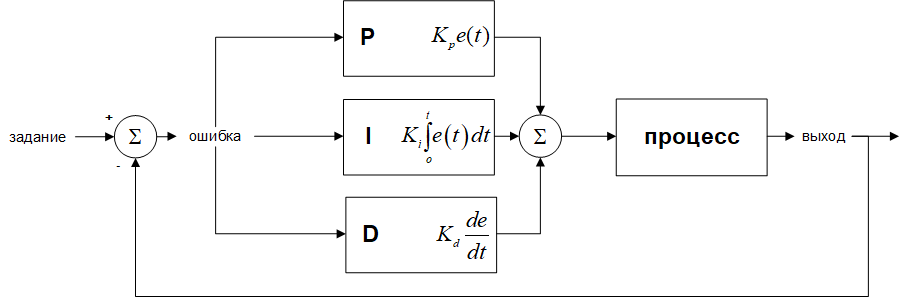
\includegraphics[width=\textwidth]{images/chapter_1/Структурная схема ПИД-регулятора.png}
    \caption{Структурная схема ПИД-регулятора}
    \label{fig:PID_controller_scheme}
\end{figure}

\subsection{Описание ПИД-регуляторов}

Назначение ПИД-регулятора – в поддержании заданного значения $x_0$ некоторой величины $x$ с помощью изменения другой величины $u$. Значение $x_0$ называется заданием, а разность $e = (x_0 - x)$ – невязкой или рассогласованием. Выходной сигнал контроллера $u$ определяется тремя слагаемыми:

\begin{equation}
    \label{eq_PID}
    u(t) = P + I + D = K_P e(t) + K_I \int_{0}^{t} e(t) dt + K_D \frac{de}{dt}
\end{equation}

где $K_P, K_I, K_D$ – коэффициенты усиления пропорциональной, интегральной и дифференциальной составляющих контроллера, соответственно.
Большинство методов настройки ПИД-регулятора используют несколько иную формулу для выходного сигнала, в которой на пропорциональный коэффициент усиления умножены также интегральная и дифференциальная составляющие:

\begin{equation}
    u(t) = K_P \left( e(t) + \frac{1}{T_I} \int_{o}^{t} e(\tau) d \tau +T_D \frac{de}{dt}\right).
\end{equation}

\textbf{Пропорциональная составляющая} – $K_P$ – вырабатывает выходной сигнал, который стабилизирует отклонение регулируемой величины. Выходной сигнал пропорциональной составляющей тем больше, чем сильнее регулируемая величина отклоняется от задания. Если входной сигнал равен заданию, то выходной равен нулю.

При использовании пропорционального контроллера значение регулируемой величины никогда не стабилизируется на заданном значении. Существует так называемая статическая ошибка, которая равна такому отклонению регулируемой величины, которое обеспечивает выходной сигнал, стабилизирующий выходную величину именно на этом значении. Например, в контроллере температуры выходной сигнал (мощность нагревателя) постепенно уменьшается при приближении температуры к заданию, и система стабилизируется при мощности равной тепловым потерям. Температура не может достичь задания, так как в этом случае мощность нагревателя станет равна нулю, и он начнет остывать.

Чем больше коэффициент пропорциональности между входным и выходным сигналом (коэффициент усиления), тем меньше статическая ошибка, однако при слишком большом коэффициенте усиления могут начаться автоколебания, а при дальнейшем увеличении коэффициента система может потерять устойчивость.

Для устранения статической ошибки используют \textbf{интегральную составляющую} – $K_I$. Она позволяет регулятору «учиться» на предыдущем опыте. Если система не испытывает внешних возмущений, то через некоторое время регулируемая величина стабилизируется на заданном значении, сигнал пропорциональной составляющей будет равен нулю, а выходной сигнал будет полностью обеспечивать интегральная составляющая.

\textbf{Дифференциальная составляющая} – $K_D$ – противодействует предполагаемым отклонениям регулируемой величины, которые могут произойти в будущем. Эти отклонения могут быть вызваны внешними возмущениями или запаздыванием воздействия регулятора на систему. Чем быстрее регулируемая величина отклоняется от задания, тем сильнее противодействие, создаваемое дифференциальной составляющей.

\subsection{Достоинства и недостатки ПИД-регуляторов}

Установление связей между параметрами и управление действиями системы может осуществляться инженерами-практиками и операторами.
Кроме того, за последние десятилетия разработано несколько методов настройки ПИД-регуляторов.

Однако, наряду с вышеуказанными достоинствами, ПИД-регуляторы имеют и ряд недостатков. Так, если рабочая точка процесса изменяется из-за возмущений, параметры контроллера требуется перенастраивать вручную, чтобы получить новую оптимальную настройку. Настройка должна осуществляться опытным оператором. Для систем с взаимодействующими контурами это процедура может быть сложной и занимать много времени. Кроме того, для процессов с переменными параметрами, временными задержками, существенными нелинейностями и значительными помехами использование ПИД-регуляторов может не обеспечить оптимальных характеристик.

Методы настройки ПИД-регуляторов также имеют ряд недостатков.
Одна из идей повышения эффективности ПИД-регуляторов заключается в управлении с самонастройкой, в котором параметры контроллера настраивались бы в оперативном режиме.

\subsection{Дискретная реализации ПИД-регулятора}

Идеализированное уравнение ПИД-регулятора (\ref{eq_PID}) является непрерывным, т. е. использует непрерывное время. При построении регулятора на базе компьютера входные и выходные переменные регулятора необходимо квантовать по времени с некоторым шагом $T_0$, и преобразовать в цифровую форму с помощью аналого-цифровых и цифро-аналоговых преобразователей. При этом уравнение ПИД-регулятора должно быть преобразовано в разностное с помощью замены производных конечной разностью, а интеграла – конечной суммой. В зависимости от выбранного метода перехода от непрерывных операторов к их дискретным аналогам возникает несколько различных уравнений, описывающих дискретные ПИД-регуляторы. При использовании метода прямоугольников для замены интеграла конечной суммой получим \cite{PID_NIL_AP}:


\begin{equation}\label{eq_discrete_PID}
    u_k = K\left[ e_k + \frac{T_0}{T_I} \sum_{i = 0}^{k} {e_{i - 1}} + \frac{T_D}{T_0} (e_k - e_{k - 1})\right],
\end{equation}

где $k = 0, 1, \ldots\frac{t}{T_0}$ - порядковый номер отсчета дискретного времени.

Недостатком такого представления уравнения регулятора является необходимость помнить значения отклонений $e_k$ для всех моментов времени от начала процесса регулирования.

Этот недостаток можно устранить, если для вычисления текущего значения управляющей переменной $u_k$ использовать ее предыдущее значение $u_{k - 1}$ и поправочный член. Для получения такого рекуррентного алгоритма достаточно вычесть из уравнения (\ref{eq_discrete_PID}) следующее уравнение \cite{PID_NIL_AP}:

\begin{equation}
        u_{k - 1} = K \left[e_{k - 1} + \frac{T_0}{T_I} \sum_{i=0}^{k-1}{e_{i - 1}}+\frac{T_D}{T_0}(e_{k - 1} - e_{k - 2})\right].
\end{equation}

В результате получим [6]:

\begin{equation}
    u_k - u_{k - 1} = q_0 e_k + q_1 e_{k - 1} + q_2 e_{k - 2},
\end{equation}

Где

\begin{equation}
    q_0=\mathbf{K}\left(1+\frac{T_D}{T_0}\right),
\end{equation}

\begin{equation}
    q_1=-\mathbf{K}\left(1+2\frac{T_D}{T_0}-\frac{T_0}{T_I}\right),
\end{equation}

\begin{equation}
    q_2=\mathbf{K}\frac{T_D}{T_0}.
\end{equation}

Таким образом, для вычисления текущего значения управляющего воздействия $u_k$ на объект управления достаточно хранить в памяти только величины $u_{k - 1}$, $e_k$, $e_{k - 1}$, $e_{k - 2}$.

Итак, алгоритм работы ПИД-регулятора может быть представлен в следующем виде [3]:

\begin{equation}\label{PID_algorithm}
    \begin{gathered}
    u_k = u_{k - 1} + \Delta u_k, \\
    \Delta u_k = q_0 e_k + q_1 e_{k - 1} + q_2 e_{k - 2}, \\
    q_0 = \mathbf{K}\left(1 + \frac{T_D}{T_0}\right), q_1 = -\mathbf{K}\left(1 + 2\frac{T_D}{T_0} - \frac{T_0}{T_I}\right), q_2 = \mathbf{K}\frac{T_D}{T_0}.
    \end{gathered}
\end{equation}

При переходе от непрерывных операторов к дискретным возникает погрешность, величина которой пропорциональна остаточному члену ряда Тейлора функции $e\left(t\right)$. Поэтому полученные дискретные уравнения можно считать эквивалентными непрерывным только при условии, что $e\left(t\right)$ изменяется слабо в пределах такта квантования. Однако с помощью аппарата z-преобразования можно показать, что основные свойства ПИД-регулятора сохраняются и при больших шагах квантования, если параметры регулятор $q_0$, $q_1$, $q_2$ выбирать не на основании параметров его непрерывного аналога, а независимо от них, методами параметрической оптимизации, выбрав необходимый критерий качества оптимизации исходя из цели регулирования. Такт квантования выбирают аналогично \cite{PID_NIL_AP}.

\section{Нейроуправление}

Нейроуправление – одно из основных направлений применения искусственных нейронных сетей. Для того чтобы алгоритмы управления могли применяться на практике, они должны быть достаточно простыми для реализации и понимания, обладать способностью к обучению, гибкостью, устойчивостью, нелинейностью. Таким образом, нейронные сети из-за своей способности обучаться на основе соотношения «вход-выход», нелинейными обобщающими способностями пригодны для решения задач управления, которые принципиально связаны с нелинейными характеристиками.

\subsection{Нейронные сети как основа построения нейрорегуляторов}

Несмотря на большое разнообразие вариантов нейронных сетей, все они имеют общие черты. Так, все они, так же, как и мозг человека, состоят из большого числа связанных между собой однотипных элементов – нейронов, которые имитируют нейроны головного мозга (рис. \ref{fig:neuron_scheme}).

\begin{figure}[H]
    \centering
    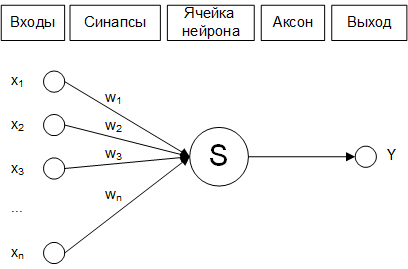
\includegraphics{images/chapter_1/Схема нейрона.png}
    \caption{Схема нейрона}
    \label{fig:neuron_scheme}
\end{figure}

Из рисунка видно, что искусственный нейрон, так же, как и живой, состоит из синапсов, связывающих входы нейрона с ядром; ядра нейрона, которое осуществляет обработку входных сигналов и аксона, который связывает нейрон с нейронами следующего слоя. Каждый синапс имеет вес, который определяет, насколько соответствующий вход нейрона влияет на его состояние. Текущее состояние нейрона определяется, как взвешенная сумма его входов:

\begin{equation}
    s = \sum_{i=1}^{n}{x_i w_i}.
\end{equation}

Выход нейрона есть функция его состояния:

\begin{equation}
    y = f(s).
\end{equation}

Нелинейная функция f называется функцией активации и может иметь различный вид (рис. \ref{fig:neuron_activation_functions}).

\begin{figure}[H]
    \centering
    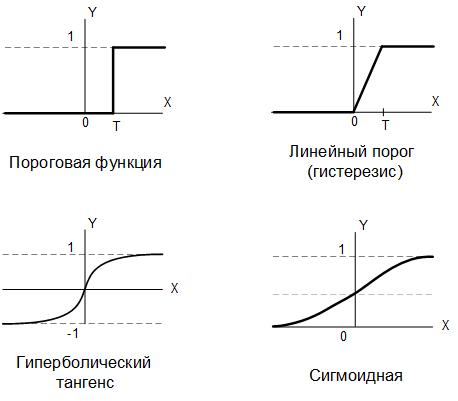
\includegraphics{images/chapter_1/Функции активации нейронов.png}
    \caption{Функции активации}
    \label{fig:neuron_activation_functions}
\end{figure}

Одной из наиболее распространенных является нелинейная функция с насыщением, так называемая сигмоидная функция:

\begin{equation}
    f(x) = \frac{1}{1 + e^{-\alpha x}}.
\end{equation}

Возвращаясь к общим чертам, присущим всем НС, отметим принцип параллельной обработки сигналов, который достигается путем объединения большого числа нейронов в так называемые слои и соединения определенным образом нейронов различных слоев, а также, в некоторых конфигурациях, и нейронов одного слоя между собой, причем обработка взаимодействия всех нейронов ведется послойно. В качестве примера простейшей НС рассмотрим трехнейронный персептрон (рис. \ref{fig:neuron_3x}), то есть такую сеть, нейроны которой имеют пороговую активационную функцию.

\begin{figure}[H]
    \centering
    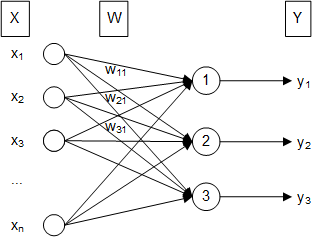
\includegraphics{images/chapter_1/Трехнейронный персептрон.png}
    \caption{Однослойный персептрон}
    \label{fig:neuron_3x}
\end{figure}

На $n$ входов поступают некие сигналы, проходящие по синапсам на $3$ нейрона, образующие единственный слой этой НС и выдающие три выходных сигнала:

\begin{equation}
    y_j = f\left[\sum_{i=1}^{n}{x_i w_{i j}}\right], j = 1..3.
\end{equation}

Очевидно, что все весовые коэффициенты синапсов одного слоя нейронов можно свести в матрицу $W$, в которой каждый элемент $w_{i j}$ задает величину $i$-ой синаптической связи $j$-го нейрона. Таким образом, процесс, происходящий в НС, может быть записан в матричной форме:

\begin{equation}
    Y = F(X W),
\end{equation}

где $X$ и $Y$ – соответственно входной и выходной сигнальные векторы, $F(V)$ – активационная функция, применяемая поэлементно к компонентам вектора $V$.

Теоретически число слоев и число нейронов в каждом слое может быть произвольным. Подробно рассмотрим алгоритм обучения многослойных нейронных сетей – алгоритм обратного распространения ошибки.

\subsection{Математические основы алгоритма обратного распространения ошибки}

\textbf{Алгоритм обратного распространения ошибки} является эффективным средством для обучения многослойных нейронных сетей.

Рассмотрим нейронную сеть, состоящую из четырех слоев (рис. \ref{fig:neural_network_4x}).

\begin{figure}[H]
    \centering
    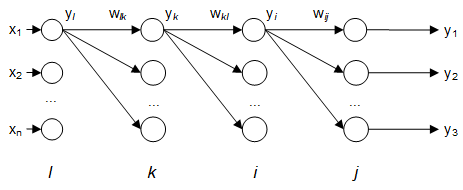
\includegraphics{images/chapter_1/Четырехслойная нейронная сеть.png}
    \caption{Четырехслойная нейронная сеть}
    \label{fig:neural_network_4x}
\end{figure}

Обозначим слои нейронных элементов от входа к выходу соответственно через $l$, $k$, $i$, $j$. Тогда выходное значение $j$-го нейрона последнего слоя равняется:

\begin{equation}
    y_j = F(S_j),
\end{equation}

\begin{equation}
    S_j = \sum_{i}{\omega_{i j} y_i - T_j},
\end{equation}

где $S_j$ — взвешенная сумма $j$-го нейрона выходного слоя; $y_i$ — выходное
значение $i$-го нейрона предпоследнего слоя; $\omega_{i j}$ — соответственно весовой коэффициент и порог $j$-го нейрона выходного слоя.

Аналогичным образом выходное значение $i$-го нейрона предпоследнего слоя определяется как:

\begin{equation}
    y_i = F(S_i),
\end{equation}

\begin{equation}
    S_i = \sum_{k}{\omega_{k i} y_k - T_i},
\end{equation}

Соответственно для $k$-го слоя:

\begin{equation}
    y_k = F(S_k),
\end{equation}

\begin{equation}
    S_k = \sum_{l}{\omega_{l k} x_l - T_k}.
\end{equation}

Алгоритм обратного распространения ошибки минимизирует среднеквадратичную ошибку нейронной сети. Для этого с целью настройки синаптических связей используется метод градиентного спуска в пространстве весовых коэффициентов и порогов нейронной сети. Согласно методу градиентного спуска изменение весовых коэффициентов и порогов нейронной сети происходит по следующему правилу:

\begin{equation}
    \omega_{i j}(t + 1) = \omega_{i j}(t) - \alpha\frac{\partial E}{\partial\omega_{i j}(t)},
\end{equation}

\begin{equation}
    T_j(t + 1) = T_j(t) - \alpha\frac{\partial E}{\partial T_j(t)},
\end{equation}

где $E$ — среднеквадратичная ошибка нейронной сети для одного образа.

Она определяется, как

\begin{equation}
    E = \frac{1}{2} \sum_{j}{(y_j - t_j)^2},
\end{equation}

где $t_j$ — эталонное выходное значение $j$-го нейрона.

Ошибка $j$-го нейрона выходного слоя равняется:

\begin{equation}
    \gamma_j = y_j - t_j.
\end{equation}

\textbf{Теорема.} Для любого скрытого слоя $i$ ошибка $i$-го нейронного элемента определяется рекурсивным образом через ошибки нейронов следующего слоя $j$:

\begin{equation}
    \gamma_i = \sum_{j = 1}^{m}{\gamma_j F^\prime(S_j)\omega_{i j},}
\end{equation}

где $m$ — количество нейронов следующего слоя по отношению к слою $i$; $\omega_{i j}$ — синаптическая связь между $i$-м и $j$-м нейроном различных слоев; $S_j$ — взвешенная сумма $j$-го нейрона.

\textbf{Теорема.} Производные среднеквадратичной ошибки по весовым коэффициентам и порогам нейронных элементов для любых двух слоев $i$ и $j$ многослойной сети определяются следующим образом:

\begin{equation}
    \frac{\partial E}{\partial\omega_{i j}} = -\gamma_j F^\prime(S_j) y_i,
\end{equation}

\begin{equation}
    \frac{\partial E}{\partial T_j} = \gamma_j F^\prime(S_j).
\end{equation}

\textbf{Следствие:} для минимизации среднеквадратичной ошибки сети весовые коэффициенты и пороги нейронных элементов должны изменяться с течением времени следующим образом:

\begin{equation}
    \omega_{i j}(t + 1) = \omega_{i j}(t) - \alpha\gamma_jF^\prime(S_j) y_i,
\end{equation}

\begin{equation}
    T_j(t + 1) = T_j(t) + \alpha\gamma_jF^\prime(S_j),
\end{equation}

где $\alpha$ — скорость обучения.

Данное следствие является очевидным. Оно определяет правило обучения многослойных нейронных сетей в общем виде, которое называется \textbf{обобщенным дельта правилом \cite{Golovko_2001}}.

\subsection{Обобщенное дельта правило для сигмоидной функции активации нейронных элементов}

Выходное значение $j$-го нейронного элемента определяется следующим образом:

\begin{equation}
    y_j = \frac{1}{1 + e^{-S_j}},
\end{equation}

\begin{equation}
    S_j = \sum_{i} {\omega_{i j} y_i - T_j}.
\end{equation}

Тогда:

\begin{equation}
    F^\prime(S_j) = \frac{\partial y_j}{\partial S_j} = y_j(1 - y_j).
\end{equation}

В результате обобщенное дельта правило для сигмоидной функции активации можно представить в следующем виде:

\begin{equation}
    \omega_{i j}(t + 1) = \omega_{i j}(t) - \alpha\gamma_j y_j (1 - y_j) y_i,
\end{equation}

\begin{equation}
    T_j(t + 1) = T_j + \alpha\gamma_j y_j(1 - y_j).
\end{equation}

Ошибка для $j$-го нейрона выходного слоя определяется, как:

\begin{equation}
    \gamma_j = y_j - t_j.
\end{equation}

Для $j$-го нейронного элемента скрытого слоя:

\begin{equation}
    \gamma_j = \sum_{i = 1}^{m}{\gamma_i y_i(1 - y_i)\omega_{j i},}
\end{equation}

где $m$ – количество нейронных элементов следующего слоя по отношению к слою $i$ (рис. \ref{fig:neuron_error}).

\begin{figure}[H]
    \centering
    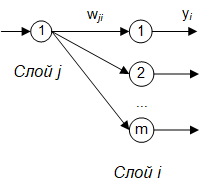
\includegraphics{images/chapter_1/Определение ошибки j-го нейронного элемента.png}
    \caption{Определение ошибки $j$-го нейронного элемента}
    \label{fig:neuron_error}
\end{figure}

\subsection{Алгоритм обратного распространения ошибки}

Как уже отмечалось, алгоритм обратного распространения ошибки был предложен в 1986 г. рядом авторов независимо друг от друга. Он является эффективным средством обучения нейронных сетей и представляет собой следующую последовательность шагов:

\begin{enumerate}[wide, labelindent=10mm]
    \item Задается шаг обучения $\alpha$ $(0 < \alpha < 1)$ и желаемая среднеквадратичная ошибка нейронной сети $E_m$.

    \item Случайным образом инициализируются весовые коэффициенты и пороговые значения нейронной сети.

    \item Последовательно подаются образы из обучающей выборки на вход нейронной сети. При этом для каждого входного образа выполняются следующие действия:

    \begin{enumerate}[wide, labelindent=20mm]
        \item производится фаза прямого распространения входного образа по нейронной сети. При этом вычисляется выходная активность всех нейронных элементов сети:

        \begin{equation}
            y_j = F(\sum_{i}{\omega_{i j}y_i - T_j)}.
        \end{equation}

        где индекс $j$ характеризует нейроны следующего слоя по отношению к слою $i$.

        \item производится фаза обратного распространения сигнала, в результате которой определяется ошибка $\gamma_j$, $j = 1, 2, \ldots$ нейронных элементов для всех слоев сети. При этом соответственно для выходного и скрытого слоев:

        \begin{equation}
            \gamma_j = y_j - t_j,
        \end{equation}

        \begin{equation}
            \gamma_j = \sum_{i}{\gamma_iF^\prime(S_i)\omega_{j i}}.
        \end{equation}

        В последнем выражении индекс $i$ характеризует нейронные элементы следующего слоя по отношению к слою $j$.

        \item для каждого слоя нейронной сети происходит изменение весовых коэффициентов и порогов нейронных элементов:

        \begin{equation}
            \omega_{i j}(t  1) = \omega_{i j}(t) - \alpha\gamma_jF^\prime(S_j)y_i,
        \end{equation}

        \begin{equation}
            T_j(t + 1) = T_j(t) + \alpha\gamma_jF^\prime(S_j).
        \end{equation}
    \end{enumerate}

    \item Вычисляется суммарная среднеквадратичная ошибка нейронной сети:

    \begin{equation}
        E = \frac{1}{2}\sum_{k = 1}^{L}{\sum_{j}{({y_j}^k} - {t_j}^k)^2},
    \end{equation}

    где $L$ — размерность обучающей выборки.

    \item Если $E>E_m$ то происходит переход к шагу 3 алгоритма. В противном случае алгоритм обратного распространения ошибки заканчивается \cite{Golovko_2001}.
\end{enumerate}

Таким образом, данный алгоритм функционирует до тех пор, пока суммарная среднеквадратичная ошибка сети не станет меньше заданной, т. е. $E\le E_m$.

\subsection{Адаптивный шаг обучения}

В стандартном алгоритме обратного распространения ошибки существует проблема выбора подходящего шага обучения, чтобы увеличить быстродействие и обеспечить сходимость алгоритма. Для выбора адаптивного шага обучения $\alpha$ можно использовать метод наискорейшего спуска. В соответствии с ним, на каждой итерации обучения нейронной сети, необходимо выбирать шаг обучения для каждого слоя таким, чтобы минимизировать среднеквадратичную ошибку сети:

\begin{equation}
    \alpha(t) = \mathbf{min}{E}(y_j(t + 1)),
\end{equation}

где $j = \overline{1, m}$, $m$ – количество нейронных элементов последнего слоя.

Выходное значение $j$-го нейрона зависит от функции активации нейронных элементов и в общем случае определяется следующим образом:

\begin{equation}
    y_j(t + 1) = F(\omega_{i j}(t + 1),T_j(t + 1)).
\end{equation}

При этом весовые коэффициенты и пороги нейронной сети модифицируются так:

\begin{equation}\label{w_ij}
    \omega_{i j}(t + 1) = \omega_{i j}(t) - \alpha(t)\frac{\partial E}{\partial\omega_{i j}(t)},
\end{equation}

\begin{equation}\label{T_j}
    T_j(t + 1) = T_j(t) - \alpha(t)\frac{\partial E}{\partial T_j(t)}.
\end{equation}

Среднеквадратичная ошибка нейронной сети равняется:

\begin{equation}
    E = \frac{1}{2}\sum_{j}{(y_j - t_j)^2.}
\end{equation}

Тогда для нахождения $\alpha(t)$ необходимо решить следующее уравнение:

\begin{equation}
    \frac{\partial E}{\partial\alpha(t)} = \frac{\partial E}{\partial y_j(t + 1)}\cdot\frac{\partial y_j(t + 1)}{\partial\alpha(t)}.
\end{equation}

Данное уравнение невозможно решить относительно $\alpha(t)$ аналитическим путем. Поэтому в ряде работ для определения адаптивного шага обучения предлагается использовать методы линейного поиска. Однако это связано со значительными вычислениями. Поэтому можно предложить приближенный метод нахождения скорости обучения $\alpha(t)$. Он базируется на разложении функции активации нейронных элементов в ряд Тейлора. Рассмотрим это подробно.

Пусть выходное значение $j$-го нейрона последнего слоя нейронной сети равняется:

\begin{equation}\label{y_j}
    y_j(t) = F(S_j(t)),
\end{equation}

\begin{equation}\label{S_j}
    S_j(t) = \sum_{i}{y_i(t)\omega_{i j}(t) - T_j}(t),
\end{equation}

где $y_i(t)$ – выходное значение $i$-го нейрона скрытого слоя.

Для определения взвешенной суммы $j$-го нейрона в момент времени $t + 1$ подставим в (\ref{y_j}) и (\ref{S_j}) выражения (\ref{w_ij}) и (\ref{T_j}):

\begin{equation}\label{S_j_t_1}
    \begin{split}
        S_j(t + 1) = \sum_{i}{y_i(\omega_{i j} - \alpha\frac{\partial E}{\partial\omega_{ij}}) - T_j + \alpha\frac{\partial E}{\partial T_j}} = \\
        \sum_{i}{y_i\omega_{i j} - T_j - \alpha\cdot(\sum_{i}{y_i\cdot\frac{\partial E}{\partial\omega_{i j}} - \frac{\partial E}{\partial T_j}})}.
    \end{split}
\end{equation}

Обозначим:

\begin{equation}\label{a_j}
    a_j = \sum_{i}{y_i\frac{\partial E}{\partial\omega_{ij}} - \frac{\partial E}{\partial T_j}}.
\end{equation}

Тогда выражение (\ref{S_j_t_1}) можно представить в следующем виде:

\begin{equation}\label{S_j_t_1_small}
    S_j(t + 1) = S_j(t) - \alpha\cdot a_j.
\end{equation}

Выходное значение $j$-го нейрона в момент времени $t + 1$ равняется:

\begin{equation}
    y_j(t + 1) = F(S_j(t + 1)).
\end{equation}

Разложим данное выражение по формуле Тейлора и ограничимся первыми двумя членами:

\begin{equation}\label{y_j_t_1}
    y_j(t + 1) = F(0) + F^\prime(0)\cdot F(S_j(t + 1),
\end{equation}

где:

\begin{equation}
    F^\prime(0) = \frac{\partial F}{\partial S_j},
\end{equation}

при $S_j = 0$.

Подставим (\ref{S_j_t_1_small}) в выражение (\ref{y_j_t_1}). Тогда:

\begin{equation}\label{y_j_t_1_mod}
    y_j(t + 1) = F(0)+F^\prime(0)S_j(t) - \alpha F^\prime(0) a_j.
\end{equation}

Так как:

\begin{equation}
    y_j(t) = F(0) + F^\prime(0)S_j(t),
\end{equation}

то выражение (\ref{y_j_t_1_mod}) можно представить в следующем виде:

\begin{equation}
    y_j(t + 1) = y_j(t) - \alpha F^\prime(0) a_j.
\end{equation}

Для определения адаптивного шага обучения необходимо обеспечить:

\begin{equation}
    E = \frac{1}{2}\sum_{j}^{\sum}{(y_j(t + 1) - t_j)^2\rightarrow\mathbf{min}}
\end{equation}

Тогда:

\begin{equation}
    \frac{\partial E}{\partial\alpha} = \sum_{j}{(y_j(t) - t_j - \alpha F^\prime(0)a_j)\cdot(-F^\prime(0) a_j) = 0}.
\end{equation}

Выражая из последнего уравнения $\alpha(t)$, получим:

\begin{equation}\label{alpha_t}
    \alpha(t) = \frac{\sum_{j}{(y_j(t) - t_j) a_j}}{F^\prime(0)\sum_{j}{a_j}^2}.
\end{equation}

Так как $\frac{\partial^2E}{\partial\alpha^2} > 0$, то при данном $\alpha(t)$ обеспечивается минимум среднеквадратичной ошибки. Найдем выражение для $a_j$. Для этого определим:

\begin{equation}\label{dE_dw}
    \frac{\partial E}{\partial\omega_{ij}} = \frac{\partial E}{\partial y_j}\cdot\frac{\partial y_j}{\partial s_j}\cdot\frac{\partial s_j}{\partial\omega_{i j}}=(y_j - t_j)F^\prime(S_j) y_i,
\end{equation}

\begin{equation}\label{de_dT}
    \frac{\partial E}{\partial T_j} = \frac{\partial E}{\partial y_j}\cdot\frac{\partial y_j}{\partial s_j}\cdot\frac{\partial s_j}{\partial T_j} = -(y_j - t_j)F^\prime(S_j).
\end{equation}

Подставляя (\ref{dE_dw}) и (\ref{de_dT}) в выражение (\ref{a_j}), получим:

\begin{equation}\label{a_j_mod}
    a_j = (1 + \sum_{i}{{y_i}^2)\cdot(y_j - t_j)}\cdot F^\prime(S_j).
\end{equation}

Исходя из принципа независимости слоев, предполагаем, что:

\begin{equation}\label{gamma_j}
    \gamma_j = y_j - t_j.
\end{equation}

Подставляя выражения (\ref{a_j_mod}) и (\ref{gamma_j}) в (\ref{alpha_t}), получим приближенное выражение для вычисления адаптивного шага обучения различных слоев нейронной сети:

\begin{equation}\label{alpha_t_final}
    \alpha(t) = \frac{\sum_{j}{{\gamma_j}^2F^\prime(S_j)}}{F^\prime(0)\cdot(1 + \sum_{j}{{\gamma_j}^2(F^\prime(S_j))^2}},
\end{equation}

где $\gamma_j$ - ошибка $j$-го нейронного элемента \cite{Golovko_2001}.

\subsection{Адаптивный шаг обучения для сигмоидной функции активации нейронных элементов}

Рассмотрим определение выражения (\ref{alpha_t_final}) для сигмоидной функции активации нейронных элементов.

Так как производные сигмоидной функции:

\begin{equation}
    {y_j}^\prime = F^\prime(S_j) = y_j(1 - y_j),
\end{equation}

\begin{equation}
    {y_j}^\prime(0) = F^\prime(0) = \frac{1}{4},
\end{equation}

то выражение для адаптивного шага обучения можно представить в следующем виде:

\begin{equation}
    \alpha(t) = \frac{4\sum_{j}{{\gamma_j}^2y_j(1 - y_j),}}{(1 + \sum_{i}{{y_i}^2)\cdot\sum_{j}{{\gamma_j}^2{y_j}^2(1 - y_j)^2}}},
\end{equation}

где ошибка $j$-го нейронного элемента скрытого слоя равняется:

\begin{equation}
    \gamma_j = \sum_{i}\gamma_i y_i(1 - y_i)\omega_{j i}.
\end{equation}

Здесь $i$ характеризует нейроны следующего слоя по отношению к слою $j$.

Заметим, что в приведенных выше выражениях $\alpha(t)$ вычисляется отдельно для каждого слоя нейронной сети. Как показывают эксперименты, при использовании адаптивного шага обучения могут получаться слишком большие значения $\alpha(t)$. Это может привести к десинхронизации процесса обучения, когда весовые коэффициенты резко изменяются в определенном направлении. В результате изменение среднеквадратичной ошибки с течением времени будет иметь колебательный характер. Поэтому рекомендуется ограничивать $\alpha(t)$ по абсолютному значению. Полученные выше выражения для адаптивного шага обучения позволяют значительно повысить скорость обучения нейронной сети и избежать выбора подходящего шага. Это является существенным преимуществом по сравнению со стандартным алгоритмом обратного распространения ошибки. Хотя при удачном выборе постоянного шага обучения данный алгоритм будет сходиться не быстрее, чем метод градиентного спуска \cite{Golovko_2001}.

\section{Классификация и обзор нейросетевых приемов управления}

В настоящее время существует большое количество подходов к нейронному управлению, однако единой четкой классификации не существует. Согласно \cite{Omatu_Khalid_Yusof}, \cite{Notkin_2006}, \cite{White_1992} можно выделить:

\begin{itemize}
    \item Последовательная схема управления. Нейронная сеть непосредственно обучается отображению желаемых (опорных) сигналов в управляющие воздействия, необходимые для получения таких сигналов.
    \item Параллельная схема управления. Нейронная схема используется для компенсации управляющего воздействия, задаваемого обычным контроллером. Компенсация производится таким образом, чтобы выходной сигнал объекта управления поддерживался как можно ближе к желаемому.
    \item Схема управления с самонастройкой. Нейронная сеть настраивает параметры управления, задающие работу обычного контроллера, таким образом, чтобы выходной сигнал объекта управления поддерживался как можно ближе к желаемому.
    \item Схема управления с эмулятором и контроллером (схема обратного распространения во времени). Максимизируется некоторая мера полезности или эффективности во времени.
    \item Адаптивно-критическая схема. Эта схема приближена к динамическому программированию, т.е. реализации оптимального управления во времени в условиях шумов и нелинейностей.
\end{itemize}

Данная классификация имеет достаточно размытые границы, что отражено на графической иллюстрации ниже (рис. \ref{fig:neuro_control_classification}).

\begin{figure}[H]
    \centering
    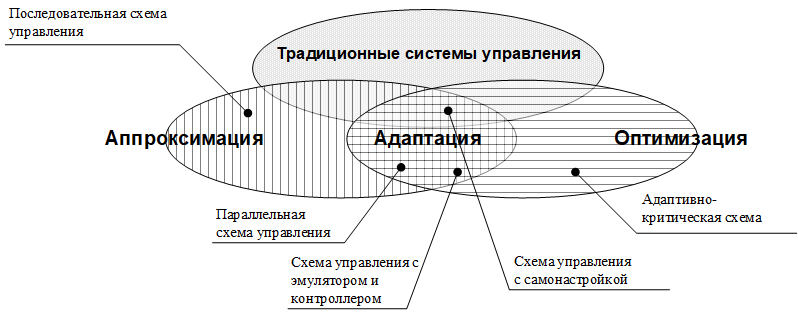
\includegraphics[width=\textwidth]{images/chapter_1/Классификация нейросетевых приемов решения задач управления.png}
    \caption{Классификация нейросетевых приемов решения задач управления}
    \label{fig:neuro_control_classification}
\end{figure}

Рассмотрим более подробно данные подходы к нейросетевому управлению.

\subsection{Последовательная схема управления}

Данная схема наиболее проста, что является как основным достоинством (несмотря на относительную простоту, подходит для решения широкого круга задач), так и недостатком (требует переобучения при изменении параметров объекта управления). Рис. \ref{fig:serial_neuro_control_scheme} отражает данную схему. Являясь одним из самых простых, данный подход имеет множество модификаций \cite{Ruano1992ApplicationsON}. Авторы Woo-Yong Han, Jin-Wook Han и Chang-Goo Lee \cite{Han1999} использовали многослойный персептрон для прогнозирования выхода системы и подстройки затем ПИД-регулятора. Другой коллектив авторов (Corneliu Lazar и др.) использовали подобный подход для надстройки выходы ПИД-регулятора \cite{Lazar2004}. Данная схема также использовалась для управления печью в работе S. Martineau и др. \cite{Martineau2003}.

\begin{figure}[H]
    \centering
    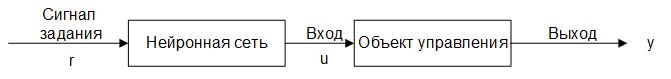
\includegraphics[width=\textwidth]{images/chapter_1/Схема последовательного нейронного управления.png}
    \caption{Схема последовательного нейронного управления}
    \label{fig:serial_neuro_control_scheme}
\end{figure}

\subsection{Схема обратного распространения во времени}

«Обратное распространение во времени» – одна из важных архитектур нейронного управления, использующая алгоритм обратного распространения ошибки. В этой схеме для управления объектом используется две нейронные сети (рис. \ref{fig:neuro_emulator_with_controller}).

\begin{figure}[H]
    \centering
    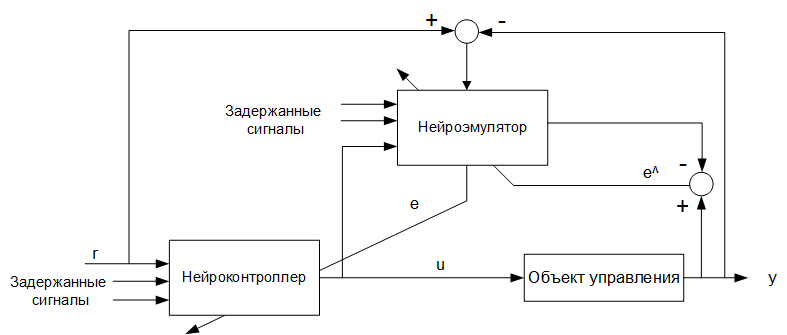
\includegraphics[width=\textwidth]{images/chapter_1/Схема нейронного обучения с эмулятором и контроллером.png}
    \caption{Схема нейронного обучения с эмулятором и контроллером}
    \label{fig:neuro_emulator_with_controller}
\end{figure}

Первая сеть используется как эмулятор, вторая – как контроллер. Сеть эмулятор может обучаться автономно, с использованием архитектуры обобщенного управления, или даже непосредственно, путем ввода случайных входных сигналов для обучения динамике объекта управления.

\subsection{Адаптивно-критическая схема}

Рассматривая подходы к обучению нейросетей, можно отдельно выделить  «обучение с подкреплением» (Reinforcement Learning) или «обучение с критикой». Необходимость применения данной парадигмы возникает в тех случаях, когда известна конечная цель, но неизвестен способ ее достижения. Это тот случай, когда желаемый отклик системы неизвестен, однако может быть дана некоторая оценка ее работы. Такая оценка обычно имеет вид скалярного «подкрепляющего» сигнала. В случае успеха он положителен, при неудаче отрицателен, а в нейтральных случаях равен нулю. Таким образом, можно поощрять за приближение к цели и наказывать за удаление от нее или за медлительность, причем поощрение может быть запаздывающим. Одной из областей применения «обучения с подкреплением» является область задач управления, когда желаемое управление на входе динамического объекта неизвестно, в то время как заметить отклонение его выхода за допустимые пределы несложно. Методы обучения с подкреплением относятся к разряду методов динамического программирования, но без модели объекта. Общая схема приведена на рис. \ref{fig:adaptive_critic_control}.

\begin{figure}[H]
    \centering
    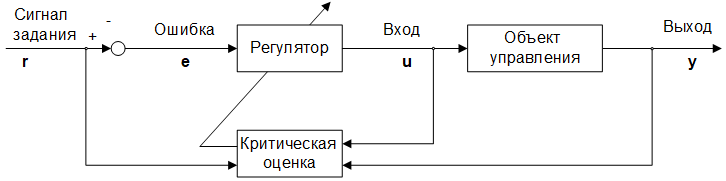
\includegraphics[width=\textwidth]{images/chapter_1/Схема адаптивно-критическая.png}
    \caption{Адаптивно-критическая схема}
    \label{fig:adaptive_critic_control}
\end{figure}

\subsection{Схема управления с самонастройкой}

В данном подходе используется настройка параметров регулятора во время работы системы. Отдельно можно выделить использование ПИД-регулятора с самонастройкой. Он может быть подстроен во время работы за счет изменения его коэффициентов. Существует большое количество схем таких самонастраивающихся ПИД-регуляторов. В данной схеме для настройки коэффициентов  используется нейронная сеть (НС).
Такие нейро-ПИД регуляторы в настоящее время используются для построения различных систем управления \cite{Omatu_Khalid_Yusof}, \cite{Omatu1997}, \cite{Omatu2010}. Рис. \ref{fig:neuro_PID_control} поясняет базовые идеи данного подхода.

\begin{figure}[H]
    \centering
    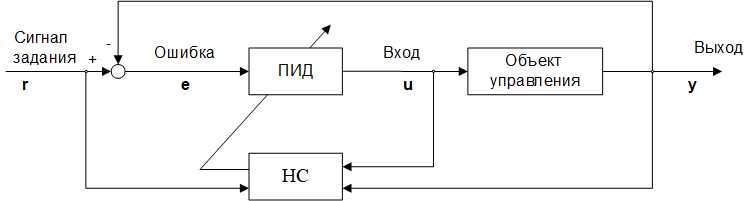
\includegraphics[width=\textwidth]{images/chapter_1/Схема neuroPID общая.png}
    \caption{Схема нейро-ПИД регулятора общая}
    \label{fig:neuro_PID_control}
\end{figure}

Обычно выходом нейронной сети являются коэффициенты ПИД-регулятора. Интересный подход используется в работе Ниша Джха \cite{Nisha2011} – весовые коэффициенты выходного слоя многослойного персептрона соответствуют коэффициентам ПИД-регулятора.

\section{Онтологии и семантические технологии}

В общем случае (отдельно от информационных технологий) слово «семантика» относится к смысловой составляющей языка – значения знаков и структур знаков. При этом семантика противопоставляется синтаксису (формальным правилам соединения знаков в текст). Если речь о семантике заводится в сфере информационных технологий, то имеют в виду особые технологии, архитектуры приложений и языки описания данных, ориентированные на знаковое представление объектов и их свойств в компьютерных моделях предметных областей. В качестве основной цели семантического подхода видится обучение компьютера распознавать смысл данных, описывающих деятельность и ее элементы, то есть реализовать переход от оперирования обезличенными данными к работе со знаниями и значениями. Предполагается, что повсеместное использование семантического подхода в моделировании предметных областей позволит унифицировать обмен информацией между независимыми поставщиками данных и приложениями, а также обеспечит возможность модифицировать структуру данных и бизнес-логику приложений не за счет переписывания кода, а только через преобразование семантически определенных данных. К основным методам семантического подхода следует отнести: унификацию формата записи, уникальную идентификацию записей, включение метаданных в данные, стандартизацию словарей.

Традиционно семантическое описание предметной области именуют онтологией этой области. При этом выражения «онтологическое описание», «онтологическая модель», «онтология предметной области» можно использовать как синонимы. Онтология или онтологическая модель предметной области – это, по сути, структура из сущностей (концептов, понятий, типов объектов), их свойств и правил установления отношений между ними. Обычно онтологию представляют в виде графа, вершинами которого являются объекты, а ребрами – свойства. Часто такую структуру из объектов и значений их свойств, построенную для определенной предметной области, называют графом знаний (Knowledge graph).

\section{Семантические технологии в управлении}

Подход к проектированию различного рода систем на основе онтологических моделей широко используется в настоящее время \cite{Боргест2010}, при этом в особую область исследований выделяют «онтологии предприятия» \cite{Шведин2010}. Суть предлагаемых подходов состоит в построении онтологий, описывающих деятельность того или иного предприятия или его подразделений. В такую систему онтологий при необходимости могут включаться знания различного рода, описывающие тот или иной аспект деятельности предприятия.

Применение онтологического подхода для структуризации знаний предприятия позволяет использовать эти знания более эффективно, в том числе, существенно облегчить процесс модернизации этих знаний, адаптации их под новые задачи, ускорить и упростить процесс обучения нового персонала \cite{Гладун2006}.

В ряде работ рассматриваются применение онтологического подхода для решения конкретных прикладных задач некоторого предприятия \cite{Загорулько2012}.

Однако для существующих онтологических моделей можно выделить ряд общих недостатков:

\begin{itemize}
    \item отсутствие единого подхода к выделению и формированию онтологий, что часто приводит к невозможности интеграции и повторного использования онтологий, разработанных в рамках одного предприятия или даже в рамках разных подразделений одного предприятия;
    \item отсутствие единого подхода к построению иерархии онтологий ограничивает возможность построения комплексной взаимосвязанной системы онтологий, описывающей предприятие на всех необходимых уровнях детализации;
    \item трудности повторного использования онтологий реального предприятия, разработанных другими, из-за их большой сложности;
    \item отсутствие удобных инструментов, поддерживающих разработку и использование онтологий.
\end{itemize}

Для решения данных проблем предлагается использовать описание в виде онтологии стандарта \textbf{ISA-88} - уровень \textbf{SCADA-систем} - на основе технологии \textbf{OSTIS}.

\section{Выводы}

В большинстве работа для «тонкой» подстройки ПИД используется многослойный персептрон (MLP). Также используются рекуррентные или RBF нейронные сети \cite{Reza2011}. Современные подходы основываются на интеграции различных подходов – нечеткой логики \cite{Tahour2007}, генетических алгоритмов \cite{Sharkawy2006}, классических подходов и т.д. \cite{Omatu_Khalid_Yusof}.
Для обучения НС обычно используется алгоритм обратного распространения ошибки (BP algorithm) \cite{Omatu_Khalid_Yusof}, \cite{Ruano1992ApplicationsON} или его модификации \cite{Han1999}. Для поиска начальных значений порогов и весовых коэффициентов используются различные подходы (например, Сигеру Омату \cite{Omatu_Khalid_Yusof} предложил использовать генетические алгоритмы). Для симуляции систем управления широко применяются пакеты MATLAB и Simulink, в некоторых работах можно встретить реализацию в качестве программного модуля для персонального компьютера (PC).

\section{Постановка задачи}

Разработать \textbf{семантический нейро-ПИД-регулятор} для использования в проектах АСУТП, также использовать описание в виде онтологии стандарта \textbf{ISA-88} - уровень \textbf{SCADA} - как часть интеллектуальной системы управления.

\chapter{Нейросетевые модели управления технологическими процессами}

В данной главе рассматриваются практические примеры применения в задачах АСУТП.

\section{Процесс пастеризации молока}

\subsection{Общие сведения}

К концу XIX века тепловая обработка молока получила столь широкое применение, что стала использоваться для разнообразных целей на большинстве молокозаводов – например, для обработки молока при изготовлении сыра и масла. До внедрения тепловой обработки молоко представляло собой постоянный источник инфекций, так как оно является идеальной средой для развития микроорганизмов. Через молоко зачастую распространялись такие болезни, как туберкулез и брюшной тиф.

В термине “пастеризация” запечатлено имя Луи Пастера, который в середине XIX века провел фундаментальные исследования воздействия тепла на микроорганизмы, приводящего к их гибели, и возможности применения температурной обработки для консервирования пищевых продуктов.

Пастеризация молока – это особый вид тепловой обработки, который можно определить как “любую тепловую обработку молока, обеспечивающую безусловное уничтожение микроорганизмов – возбудителей туберкулеза, не вызывая при этом значительных изменений физических и химических качеств молока” \cite{TetraPak1995}.

Пластинчатая пастеризационно-охладительная установка (ПОУ) предназначена для тепловой обработки и охлаждения молочных продуктов в непрерывном тонкослойном закрытом потоке. Схема типовой пастеризационной установки приведена ниже (рис. \ref{fig:POU_Tetra_Pak}). Нагрев осуществляется за счет подачи пара через управляемый клапан \textbf{VC1}. Диапазон работы управляемых паровых клапанов от $\text{0\%}$ – полностью закрыт, до $\text{100\%}$ – полностью открыт. Температура \textbf{TE1} поддерживаться в пределах $92 \pm 2 \SI{}{\celsius}$.

Современная ПОУ, включающая оборудование для эксплуатации, надзора и управления процессом, собирается из согласованных компонентов, образуя сложный технологический агрегат. Для автоматизации регулирования температурного режима в состав ПОУ входит система управления на базе промышленного контроллера. От применяемых алгоритмов управления напрямую зависит качество получаемой продукции.

\begin{figure}[H]
    \centering
    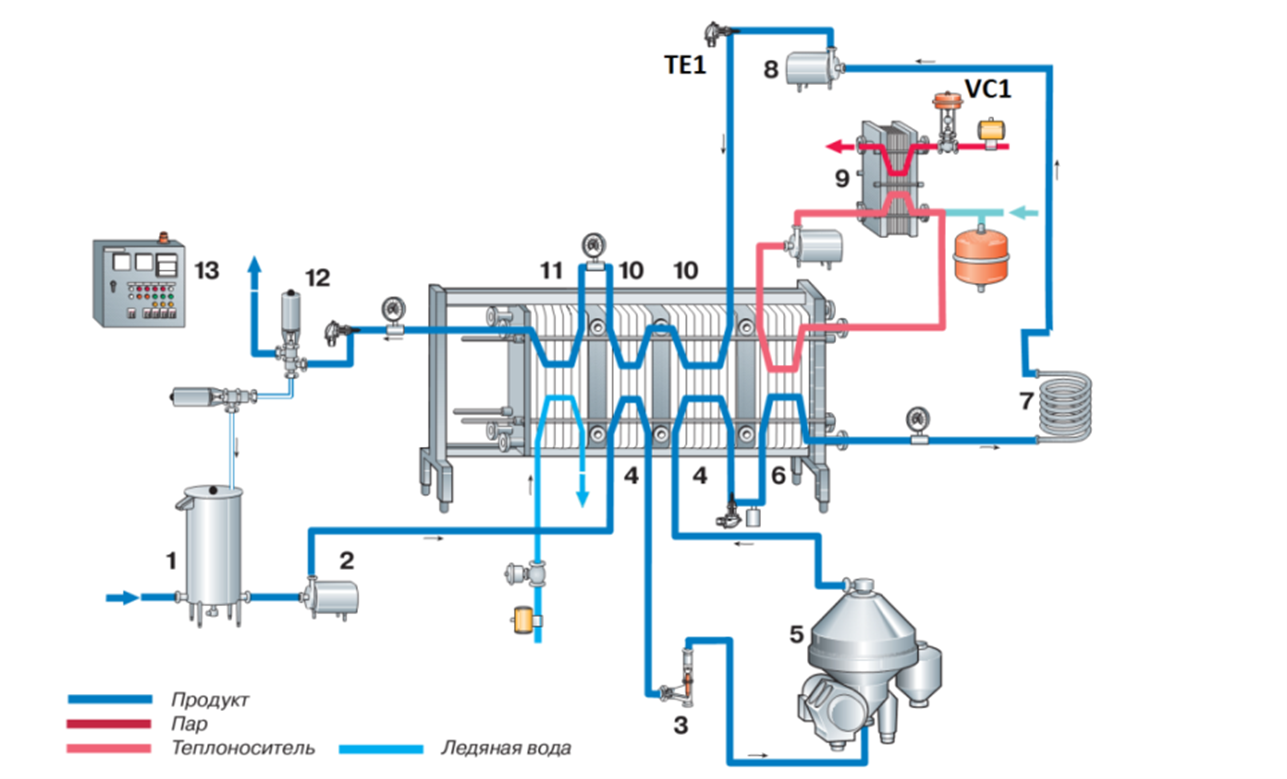
\includegraphics[width=\textwidth]{images/chapter_2/ПОУ Tetra Pak.png}
    \caption{Схема и общий вид пастеризационной установки, где: 1 - балансный танк, 2 - подающий насос, 3 - регулятор потока, 4 - секции регенеративного предварительного подогрева, 5 - центробежный очиститель, 6 - секция нагрева, 7 - труба выдержки, 8 - вспомогательный насос, 9 - система нагрева горячей воды, 10 - секции регенеративного охлаждения, 11 - секции охлаждения, 12 - клапан возвратный, 13 - панель управления}
    \label{fig:POU_Tetra_Pak}
\end{figure}

\subsection{Пастеризационные установки как объект автоматизации}

Рассмотрим подробно секцию нагрева ПОУ. Входные и выходные параметры и возмущающие воздействия для нее представлены на рис. \ref{fig:Pasterizer_heat_section}.

\begin{figure}[H]
    \centering
    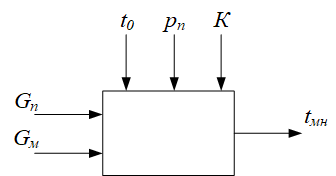
\includegraphics{images/chapter_2/Pasterizer_heat_section.png}
    \caption{Структурная схема секции нагрева ПОУ как объекта автоматизации}
    \label{fig:Pasterizer_heat_section}
\end{figure}

Основными причинами, вызывающими колебания температуры $t_\text{мн}$ нагревания молока являются непостоянство расхода $G_\text{м}$ продукта, непостоянство температуры $t_0$ исходного молока, изменение расхода $G_\text{п}$ пара, обусловленное колебания его давления $p_\text{п}$, изменение коэффициента теплопередачи $K$ вследствие отложения белка молока на теплопередающих поверхностях \cite{Вайнберг1978}.

Для стабилизации температуры $t_\text{мн}$ нагревания молока в качестве управляющего воздействия в основном применяют расход пара $G_\text{п}$. Его регулируют посредством управляемого клапана (\textbf{VC1} на рис. \ref{fig:Pasterizer_heat_section}).

Статические и динамические характеристики большинства ПОУ в настоящее время экспериментально и аналитически выявлены. Для нагревательной части по каналу $G_\text{п} \rightarrow t_\text{мн}$, т. е. зависимость $t_\text{мн}=F(G_\text{п})$ определяется из уравнения теплового баланса секции пастеризации и систем обогрева горячей воды. Если пренебречь потерями тепла в окружающую среду, то уравнение теплового баланса в установившемся режиме имеет вид:

\begin{equation}
    G_\text{м} c_\text{м}(1 - \varepsilon)(t_\text{мн} - t_0) = G_\text{п}(i - c_\text{к} t_\text{к}),
\end{equation}

где $c_\text{к}$ – температура конденсата \SI{}{\celsius}; $c_\text{м}$, $c_\text{к}$ – теплоемкость соответственно молока и конденсата, Дж/(кг·\SI{}{\celsius}); $\varepsilon$ – коэффициент регенерации тепла установки; $i$ – энтальпия пара, Дж/кг. После преобразования данного уравнения получаем статическую характеристику нагревательной части установки:

\begin{equation}
    t_\text{мн} = t_0 + \frac{i - c_\text{к} t_\text{к}}{G_\text{м} c_\text{м}(1 - \varepsilon)} G_\text{п}.
\end{equation}

Результаты экспериментальных и теоретических исследований показали, что динамическая характеристика нагревательной части установки по каналу «расход пара – температура нагрева молока» может быть выражена передаточной функцией:

\begin{equation}\label{steam_temp_relation}
    W(p) = \frac{K_\text{п} e^{-p \tau_\text{з}}} {Tp + 1},
\end{equation}

где $K_\text{п}$ – коэффициент передачи объекта, \SI{}{\celsius}/(кг/с),

\begin{equation}
    K_\text{п} = \frac{i - c_\text{к} t_\text{к}}{G_\text{м} c_\text{м}(1 - \varepsilon)},
\end{equation}

где $T$ – постоянная времени объекта, с; $\tau_\text{з}$ – время запаздывания, с; $p$ – комплексная переменная (оператор Лапласа).

Таким образом, передаточная функция нагревательной части установки характеризуется последовательно соединенными апериодическим звеном первого порядка и звеном транспортного запаздывания. В таблице \ref{table:pasterizer_params} приведены средние значения параметров некоторых ПОУ.

\begin{table} [H]
    \small
    \caption{Параметры ПОУ}\label{table:pasterizer_params}
    \centering
    \begin{tabular}{ | c | c | c | c | }
        \hline
        \textbf{Установка} & $K_\text{п}$, \SI{}{\celsius}/(кг/с) & $T$, c & $\tau_\text{з}$, c \\
        \hline
        ОПУ-5М             & 2300                                 & 369    & 12                 \\
        \hline
        ОПУ-10             & 1150                                 & 190    & 7                  \\
        \hline
        ОПУ-25             & 525                                  & 450    & 4                  \\
        \hline
    \end{tabular}
\end{table}

При накоплении белковых веществ на теплопередающих поверхностях значения $T$ в среднем возрастают на 50 - 60\%.

\subsection{Компьютерное моделирование процесса пастеризации}

Для компьютерного моделирования получим дискретную модель процесса пастеризации на основе формулы (\ref{steam_temp_relation}).

Рассмотрим процесс без участия звена запаздывания $e^{-p \tau_\text{з}}$, положим $k = K_\text{п}$. Выберем достаточно малый шаг времени $h$ и будем вычислять значения сигналов на выходе в дискретные равноотстоящие моменты времени $t = hl$ $(l = 0, 1, 2, \ldots)$. Выходную величину определим по рекуррентным формулам квадратичной интерполяции на основе значений сигнала, полученных в предыдущие моменты времени. Дифференциальное уравнение процесса в интервале $(l - 1)h < t \le hl$ имеет вид:

\begin{equation}
    Tdy(\tau)/d\tau + y(\tau) = kx(\tau),
\end{equation}

где $\tau = t - (l - 1)h$.

При $\tau = 0$ значения $x[(l - 1)h] = x_{l - 1}, y[(l - 1)h] = y_{l - 1}$.

Переходя к изображениям по Лапласу и решая уравнение относительно $Y(p)$, получим:

\begin{equation}
    Y(p) = \frac{1}{1 + pT}y_{l - 1}+\frac{k}{1 + pT}[X(p) - x_{l - 1}].
\end{equation}

При использовании квадратичной интерполяции сигнал $x(t)$ в интервале $[(l - 1)h, lh]$ определяется значениями $x$ для трех моментов времени $x_l = x(lh), x_{l - 1} = x[(l - 1)h)]$ и $x_{l - 2} = x[(l - 2)h)]$, т.е.:

\begin{equation}
    x(t) = x_{l - 1} + \frac{x_l - x_{l - 2}}{2h} + \frac{x_l - 2x_{l - 1}+ x_{l - 2}}{h^2},
\end{equation}

или в изображениях:

\begin{equation}
    x(p) = \frac{x_{l - 1}}{p} + \frac{x_l - x_{l - 2}}{2h}\cdot\frac{1}{p^2} + \frac{x_l - 2x_{l - 1} + x_{l - 2}}{h^2}\cdot\frac{1}{p^3}.
\end{equation}

Выполняя подстановку и обратное преобразование Лапласа, при $\tau = h$, т.е. в конце интервала $(t = lh)$, имеем:

\begin{equation}
    y_l = \gamma y_{l - 1} + Ax_l + Bx_{l - 1} + Cx_{l - 2},
\end{equation}

где:

\begin{equation}
    \begin{rcases}
        \gamma = e^{-h/T};\\
        A = \frac{k}{2h^2}[(1 - \gamma)(2T^2 - Th) + 2h^2 - 2Th];\\
        B = -\frac{k}{h^2}[(1 - \gamma)(2T^2 - h^2) + h^2 - 2Th];\\
        C = \frac{k}{2h^2}[(1 - \gamma)(2T^2 + Th) - 2Th].
    \end{rcases}
\end{equation}

С учетом запаздывания $\tau_\text{з}$ получим \cite{Нетушил1978}:

\begin{equation}
    y_l = \gamma y_{l - 1} + Ax_{l - \tau_\text{з}} + Bx_{l - \tau_\text{з} - 1} + Cx_{l - \tau_\text{з} - 2}.
\end{equation}.

\subsection{Разработанный нейро-ПИД регулятор ПОУ}

Общая структура самонастраивающегося нейро-ПИД регулятора показана на рисунке \ref{fig:neuro_PID_controller}, где выходы нейронной сети – пропорциональный ($K$) коэффициент, интегральная ($T_I$) и дифференциальная ($T_D$) составляющие.

\begin{figure}[H]
    \centering
    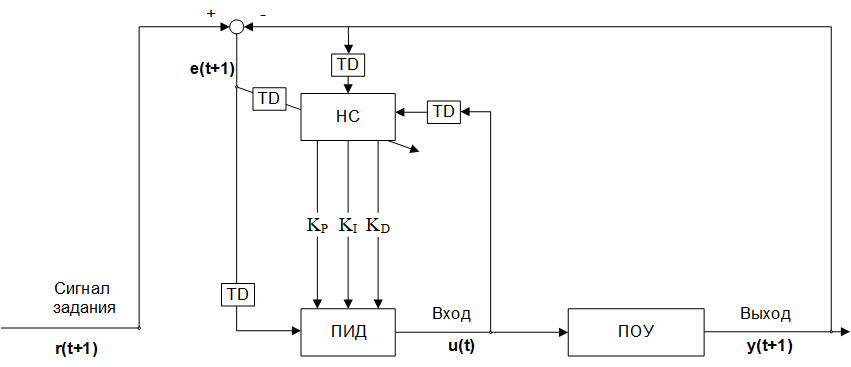
\includegraphics[width=\textwidth]{images/chapter_2/Разработанный нейро-контроллер.png}
    \caption{Разработанный нейро-ПИД-регулятор, TD означает оператор задержки}
    \label{fig:neuro_PID_controller}
\end{figure}

В качестве настройщика ПИД использовался многослойный персептрон (MLP) со следующей структурой: 20 входных, 10 скрытых и 3 выходных нейронных элемента; функция активации скрытого и выходного слоев – сигмоидная (рис. \ref{fig:PID_neuro_tuner}).

\begin{figure}[H]
    \centering
    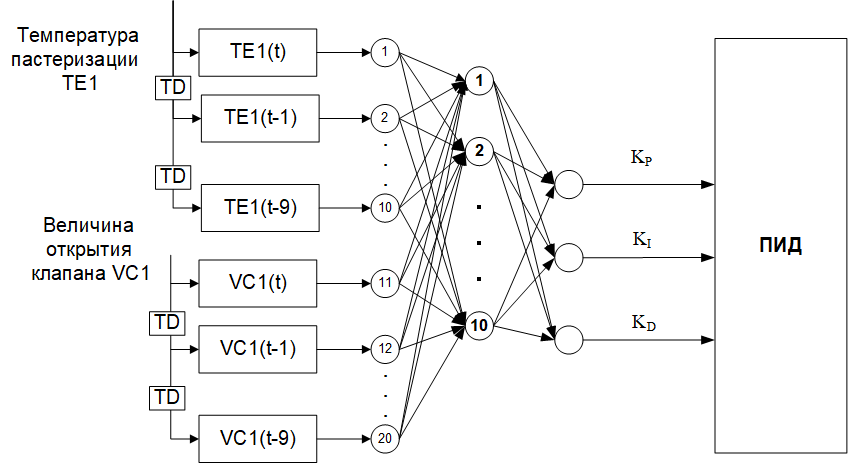
\includegraphics[width=\textwidth]{images/chapter_2/Нейро-настройщик ПИД.png}
    \caption{Нейро-настройщик ПИД}
    \label{fig:PID_neuro_tuner}
\end{figure}

\subsection{Алгоритм функционирования нейро-ПИД регулятора}

ПИД-регулятор в дискретном времени можно описать выражением \ref{PID_algorithm}, где $P$, $T_I$ и $T_D$ – пропорциональный коэффициент, интегральная и дифференциальная составляющие соответственно, $u_n$ определяет вход объекта управления в момент времени $t = n T_0$ и $e_n$ – ошибка между желаемым значением выхода $r_n$ и реальным, то есть $e_n = r_n - y_n$. $T_0$ определяет единичный интервал времени.

Для использования алгоритма обратного распространения ошибки мы должны выбрать функцию $E$, значение которой должно быть минимизировано. В качестве такой функции будет выступать ошибка управления $e_n$ в момент времени $t = n T_0$ - получаем $E_n = \frac{1}{2}e_n^2$.
Для накопления ошибок сохраняем полученные ранее данные – $E_{n-p},...E_{n-2},E_{n-1},E_n$, где $p$ определяет количество сохраненных ранее образов, используемых для обучения сети.


\chapter{Онтологические модели управления технологическими процессами}

\section{Общее описание}

Важную роль играют все участники процесса: пользователи — люди (операторы, мастера, начальники цеха и т.п.); устройства — датчики и исполнительные механизмы (температурные датчики, насосы, клапана и т.п.); механизированные системы — конвейерные системы, агрегаты; роботизированные системы — шарнирные роботы, дельта-роботы, манипуляторы; так и программные системы — SCADA, MES, ERP. Их взаимодействие обеспечивает достижение поставленной цели, устранение и предотвращение внештатных ситуаций. Причем важное влияние имеют как количественные показатели (количество операторов, устройств, агрегатов, панелей управления и т.п.), так и качество (качество устройств, квалификация операторов, качество программных систем и т.п.). В системах управления также важным является такой параметр, как скорость принятия решений — оперативное внесение изменений для выполнения поставленных планов. Онтологическое описание позволяет получить общее описание, понятное всем данным участникам процесса.
Ключевым фактором, препятствующим появлению систем автономного интеллектуального производства уже сегодня, является отсутствие общего архитектурного подхода к созданию цифровых платформ управления производствами, с одной стороны, и «зоопарк» форматов и стандартов работы с данными — с другой. Примечательно, что на эти два вызова уже существуют технологические ответы, которые получили общее название «индустриальные графы знаний» \cite{Муромцев2019} и показывают преимущества онтологического подхода, обеспечивающего гибкое моделирование и интероперабельность данных, стек семантических технологий, позволяющий выполнять анализ неструктурированной информации и интеллектуальный поиск данных во множестве разнородных источников, а также машинное обучение, обеспечивающее анализ и классификацию данных, в том числе в условиях неполной информации.

Анализ работ позволил сформулировать наиболее важные и распространенные проблемы, связанные с разработкой и применением современных стандартов в различных областях \cite{Серенков2004, Углев2012}:

\begin{itemize}
    \item Прежде всего, сложность ведения самих стандартов из-за дублирования информации, особенно сложности изменения терминологии.
    \item Дублирование информации в документации, описывающей стандарт.
    \item Проблемы интернационализации стандартов — перевод стандарта на несколько языков фактически требует поддержки и согласования независимых версий стандарта на разных языках.
    \item Как следствие — несоответствия в формате разных стандартов. Также усложняется автоматизация процесса разработки и применения стандартов.
    \item Неудобство использования стандарта, особенно сложность поиска нужной информации. Как следствие — сложность изучения стандартов.
    \item Сложность автоматизации проверки соответствия объекта или процесса требованиям конкретного стандарта.
    \item и т. д.
\end{itemize}

\section{Краткая характеристика ISA стандартов в АСУТП}

Эти проблемы в основном связаны с представлением стандартов. Наиболее перспективным подходом к решению этих проблем является преобразование каждого конкретного стандарта в базу знаний, которая базируется на наборе онтологий, соответствующих этому стандарту \cite{Серенков2004, Углев2012}. Такой подход позволяет существенно автоматизировать процессы разработки стандарта и его применения.

В качестве примера рассмотрим стандарт \textbf{\textit{ISA-88}} \cite{ISA88} (базовый стандарт для серийного производства). Хотя этот стандарт широко используется американскими и европейскими компаниями и активно внедряется на территории Республики Беларусь, он имеет ряд недостатков. Основными стандартами серийных систем ISA являются:

\begin{itemize}
    \item \textit{ANSI/ISA-88.00.01-2010}, Batch Control -- Part 1: Models and Terminology;
    \item \textit{ISA-88.00.02-2001}, Batch Control -- Part 2: Data Structures and Guidelines for Languages;
    \item \textit{ANSI/ISA-TR88.00.02-2015}, Machine and Unit States: An implementation example of \textit{ANSI/ISA-88.00.01};
    \item \textit{ISA-88.00.03-2003}, Batch Control -- Part 3: General and Site Recipe Models and Representation;
    \item \textit{ISA-TR88.0.03-1996}, Possible Recipe Procedure Presentation Formats;
    \item \textit{ANSI/ISA-88.00.04-2006}, Batch Control -- Part 4: Batch Production Records;
    \item \textit{ISA-TR88.95.01-2008}, Using ISA-88 and ISA-95 Together;
    \item \textit{IEC 61512-1}, The European version approved in 1997, based on the older version \textit{ISA-88.01-1995};
    \item \textit{GOST R IEC 61512-1-2016} -- Russian version of the standard, identical to \textit{IEC 61512-1}.
\end{itemize}

Другим стандартом, часто используемым в контексте Industry 4.0, является \textit{\textbf{ISA-95}} \cite{ISA95}. \textit{\textbf{ISA-95}} — это отраслевой стандарт для описания систем управления высокого уровня. Его основная цель — упростить разработку таких систем, абстрагироваться от аппаратной реализации и предоставить единый интерфейс для взаимодействия со слоями ERP и MES. Состоит из следующих частей:

\begin{itemize}
    \item \textit {ANSI/ISA-95.00.01-2010}, Enterprise-Control System Integration -- Part 1: Models and Terminology;
    \item \textit {ANSI/ISA-95.00.02-2018}, Enterprise-Control System Integration -- Part 2: Objects and Attributes for Enterprise-Control System Integration;
    \item \textit {ANSI/ISA-95.00.03-2013}, Enterprise-Control System Integration -- Part 3: Activity Models of Manufacturing Operations Management;
    \item \textit {ANSI/ISA-95.00.04-2018}, Enterprise-Control System Integration -- Part 4: Objects and Attributes for Manufacturing Operations Management Integration;
    \item \textit {ANSI/ISA-95.00.05-2018}, Enterprise-Control System Integration -- Part 5: Business-to-Manufacturing Transactions;
    \item \textit {ANSI/ISA-95.00.06-2014}, Enterprise-Control System Integration -- Part 6: Messaging Service Model;
    \item \textit {ANSI/ISA-95.00.07-2017}, Enterprise-Control System Integration -- Part 7: Alias Service Model;
    \item \textit {ANSI/ISA-95.00.08-2020}, Enterprise-Control System Integration -– Part 8: Information Exchange Profiles.
\end{itemize}

Модели помогают определить границы между бизнес-системами и системами управления. Они помогают ответить на вопросы о том, какие функции могут выполнять какие задачи и какой информацией должны обмениваться приложения. Комитет по разработке стандартов ISA5 часто называют среди практиков стандартом ISA-5.1. Однако комитет ISA5 «Documentation of Measurement and Control Instruments and Systems» имеет более широкую сферу деятельности, а именно разработку стандартов, рекомендуемых практик и технических отчетов для документирования и иллюстрации измерительных и контрольных приборов и систем, подходящих для всех отраслей. Стандарты ISA5 состоят из следующих документов:

\begin{itemize}
    \item \textit {ANSI/ISA-5.1-2022}, Instrumentation Symbols and Identification;
    \item \textit {ISA-5.9 working group}, Controller Algorithms and Performance;
    \item \textit {ISA-5.4}, Instrument Loop Diagrams;
    \item \textit {ISA-5.5-1985}, Graphic Symbols for Process Displays;
    \item \textit {ISA-5.6}, Documentation for Control Software Applications;
\end{itemize}

Этот стандарт полезен, когда требуется ссылка на оборудование в химической, нефтяной, энергетической, кондиционирующей, металлообрабатывающей и многих других отраслях промышленности. Стандарт позволяет любому человеку с достаточным уровнем знаний о заводе читать технологические схемы, чтобы понимать, как измерять и контролировать процесс, не вдаваясь в подробности приборов или знания эксперта.

\section{Анализ развития средств автоматизации производства предприятия ОАО
«Савушкин продукт»}

В конце 90-х на предприятии было принято решение разрабатывать своими силами
платформу системы, которая в дальнейшем позволяла бы реализовать не только
промышленные проекты автоматизированных систем управления технологическими
процессами (АСУТП), но и решать бухгалтерские, складские и т.п. задачи. В
разрабатываемой SCADA-системе (Supervisory Control And Data Acquisition —
диспетчерское управление и сбор данных), названной \textbf{EasyServer}, первым
был реализован проект по контролю температур в технологических ёмкостях (танках)
аппаратного цеха. После его успешного запуска и получения подтверждения
эффективности принятых решений, были реализованы проекты по автоматизации
моечной станции, цеха приёмки молока, цеха сгущения.

В ходе развития системы уровень автоматизации постоянно повышался. На начальном
этапе охватывался только сбор и протоколирование данных с датчиков (температура,
давление и т.д.). На последующем этапе появился уровень управления
технологическими операциями и техническими устройствами. В настоящее время
реализуется уровень рецептурного (партионного) производства.

Для разработки проектов используется также кроме \textbf{EasyServer} среда
разработки \textbf{CODESYS} от компании 3S-Smart Software Solutions для
контроллеров \textbf{WAGO}. Она бесплатна, позволяет использовать инженерные
языки для программируемых логических контроллеров (IEC 61131-3) – IL, LD, FBD,
SFC, ST. Такой подход используется для разработки относительно простых
автономных проектов (например, посты приёмки молока) инженером по автоматизации
без привлечения инженера-программиста. Реализованные проекты интегрируются в
систему за счёт использования открытого протокола обмена MODBUS TCP. Для
эффективной организации работы цеха требуется решение задач организации
взаимодействия между отдельными проектами. Однако нет универсального подхода – в
одних проектах используется MODBUS TCP, в других – дополнительный контроллер в
качестве коммуникационного шлюза. Кроме того, используются физические соединения
для обмена сигналами. Всё это дополнительно усложняет систему.

Использование собственной разработки (как проектов, так и системы в целом)
обладает следующими достоинствами:
\begin{itemize}
    \item Высокая скорость разработки новых проектов. Вся накопленная при
    разработке функциональность становится частью системы. В настоящее время
    типовой проект можно разработать силами буквально одного инженера по
    автоматизации в течение нескольких часов, что позволило реализовать уже
    более 200 проектов;
    \item Относительная дешевизна разработанной SCADA-системы
    \textbf{EasyServer}. Несмотря на содержание штата квалифицированных
    разработчиков, затраты на неё оказались гораздо ниже, чем при использовании
    сторонних решений;
    \item Обширный функционал собственной системы. Возможности системы
    сопоставимы с коммерческими аналогами (Simatic Step 7 + Simatic WinCC) за
    счёт тесной связи с реальным производством.
\end{itemize}

Существуют следующие недостатки текущего варианта системы автоматизации
производства:
\begin{itemize}
    \item Представление данных реализовано в форме простых отчётов. На этапе
    запуска первых проектов отчёты были реализованы в виде отдельных приложений
    на Delphi, данные из таблиц через BDE от сервера проекта экспортировались в
    MS Excel. На текущий момент принято решение организовать обработку данных (и
    формирование отчётов в том числе) на более высоком уровне, а на уровне АСУТП
    оставить только базовые отчёты о работе проектов. Поэтому открыт вопрос о
    платформе верхнего уровня (уровень предприятия в целом – ERP) для решения
    отчётных задач;
    \item Так как приоритетом является скорость разработки и модификации, имеет
    место низкий уровень документации как системы в целом, так и отдельных
    проектов. В связи с этим требуются решения, в которых документация
    становится частью проектируемой системы. В настоящее время описание
    функциональной схемы автоматизации, электрической части и спецификации
    проекта реализовано в CAD Eplan. Описание технологической части также
    выполняется с помощью CAD Eplan, но хранится отдельно в виде сценариев на
    языке \textbf{Lua}. Описание отдельных устройств (частотные преобразователи,
    клапаны) хранится в формате PDF и поступает от их производителей;
    \item Ограниченное время на тестирование и отладку. Поэтому востребованы
    модули диагностики и самодиагностики для проектов;
    \item Для успешного освоения рынка необходимо привести организацию
    производства на предприятии «Савушкин продукт» в соответствие с
    международными стандартами (в частности, со стандартом \textbf{ISA-88}).
    Однако стандарты могут являться и сдерживающим фактором – они громоздки,
    есть сложности с их толкованием, их внедрение может требовать неоправданно
    больших затрат. Поэтому для реализации процесса приведения предприятия в
    соответствие с международными стандартами необходимо использовать более
    гибкую организацию самого производства с учётом эволюции самого стандарта.
\end{itemize}

Растёт охват предприятия автоматизацией. Теперь это уже не только отдельные
цехи, но и всё предприятие в целом. Поэтому востребованы системы управления не
на уровне «оператор» – «мнемокарта техпроцесса» – «отдельный техпроцесс», а
«диспетчер производственной логистики» – «интеллектуальный веб-интерфейс» –
«завод в целом». Роботизация производства – необходимый элемент развития
современного предприятия. Поэтому нужны решения, позволяющие интегрировать и
реализовывать новые проекты роботизации производственных процессов и переходу к
безлюдному производству.

\section{Формализация стандарта ISA-88}

В системах управления знаниями с целью решения задач в проблемной области в соответствии с онтологическим подходом строится концептуальная модель этой проблемной области – предметная область [Голенков, 2013]. Для работы с ней строятся её спецификации – онтологии различного вида [Давыденко и др., 2016; Ивашенко, 2011], которые могут рассматриваться в качестве многократно используемых компонентов [Ивашенко, 2011; Голенков, 2013]. Онтологии, которые являются результатом согласования нескольких участников их разработки в рамках предприятия, могут быть отнесены к стандартам систем управления знаниями этого предприятия.
Системы управления знаниями могут использовать знания, соответствующие различным стандартам. Для систем управления знаниями серийного (рецептурного) производства существует несколько стандартов (IEC 61131/3, ISA-88, ISA-95, IEC-62264, IEC-60848, IEC-60050, IEC-19501, ISO/IEC-9075), которые относятся к разным уровням и аспектам подсистем подобных систем.
Любой стандарт можно рассматривать как онтологию, которая в свою очередь состоит из множества онтологий, которые могут быть структурированы как иерархия онтологий. В соответствии с моделью спецификации знаний [Ивашенко, 2015], может быть выстроена формальная модель онтологии [Гаврилова, 2000], соответствующая формальной модели стандарта. Выстроенная формальная модель онтологии задаёт онтологию, являющуюся результатом формализации такого стандарта, т.е. результатом «понимания» стандарта содержащей её системой. С целью формализации необходимо произвести анализ документа стандарта, сформировать первичную формальную модель онтологии, носитель которой включает значимые элементы исходного документа, а сигнатура – их отношения и функции, соответствующие пониманию этого стандарта в той или иной семантике. Далее, в соответствии с моделью спецификации знаний, необходимо построить соответствующие онтологию и её формальную модель в семантике системы управления знаниями предприятия. В случае предлагаемого подхода – в семантике модели унифицированного семантического представления знаний – модельной семантике ситуативных множеств [Ивашенко, 2013]. Так как выстраиваемая онтология рассматривается как часть базы знаний [Ивашенко, 2009, Давыденко и др., 2016] системы управления знаниями, то порядок формирования этих онтологий и их формальных моделей может соответствовать различным методикам [Ивашенко, 2011] и моделям проектирования [Давыденко, 2016] баз знаний.
В случае готового документа, такого как стандарт, можно использовать методику концептуального или структурного проектирования [Ивашенко, 2011].

В последнем случае формализация состоит из этапов следующих классов, которые соответствуют явным формулировкам задач процесса проектирования базы знаний:
\begin{itemize}
    \item анализ содержания документа, спецификация его структуры и выделение разделов и подразделов до атомарных (элементарных);
    \item формирование спецификации каждого раздела, описываемых в них (значимых, ключевых) элементов и соответствующих предметных областей. Каждая предметная область специфицируется набором онтологий, описывающих соответствующий вид знаний:
    \begin{itemize}
        \item терминологическая онтология;
        \item теоретико-множественная онтология;
        \item логическая онтология;
        \item онтология задач и решений задач;
        \item и другие;
    \end{itemize}
    \item оформление сформированных спецификаций предметных областей в виде разделов, верификация и интеграция их в общую иерархию структур (разделов) базы знаний.
\end{itemize}

Последние два класса этапов повторяются, пока все задачи не будут решены. Количество этапов и перечень соответствующих задач может уточняться в процессе формализации стандарта.
В результате выполнения первого этапа получена иерархия разделов, включающая декомпозицию на подразделы. Каждая часть стандарта соответствует своему разделу. Для каждого формализуемого раздела выделены его ключевые элементы, так например, раздел «Definitions» («Термины и определения») второй части документа «Data structures and Guidelines for Languages» («Структуры данных и руководство по языку») имеет не менее восьми ключевых элементов. Для каждого такого ключевого элемента указаны термины на соответствующих языках, например, «recipe entity» («рецептурная сущность») (Рис. \ref{fig:recipe_entity_main_scg}), в случае наличия синонимов, например, для «соединительное звено» («link»), указывается каждый из них (Рис. \ref {fig:recipe_entity_synonym_scg}). Способность предлагаемого подхода различать понятия и термины, позволяет легко адаптировать систему к разным языкам и конкретным пользователям или вносить изменения в стандарт, связанные с неоднозначностью употребления терминов на практике или сменой терминологии при обновлении стандарта.

\begin{figure}[H]
    \centering
    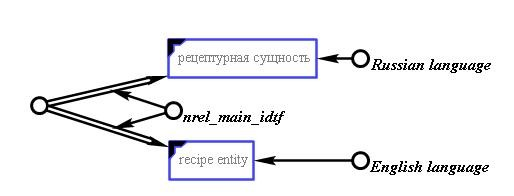
\includegraphics{images/chapter_3/рецептурная_сущность_главная_scg.jpg}
    \caption{Указание терминов ключевых элементов}
    \label{fig:recipe_entity_main_scg}
\end{figure}

\begin{figure}[H]
    \centering
    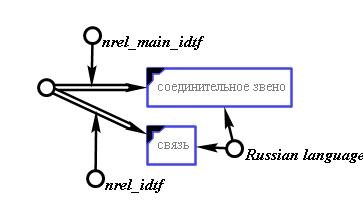
\includegraphics{images/chapter_3/рецептурная_сущность_синоним_scg.jpg}
    \caption{Указание синонимичных терминов}
    \label{fig:recipe_entity_synonym_scg}
\end{figure}

Другими ключевыми элементами в разделах документа являются:
\begin{itemize}
    \item обзорная модель (overview model),
    \item модель процессов (process model),
    \item модель технологического управления (procedural control model),
    \item модель рецептур (recipe model),
    \item физическая модель (physical model),
    \item модель оборудования (equipment model),
    \item модель деятельности управления (control activity model),
    \item планы рецептурного производства (batch schedule),
    \item история рецептурного производства (batch history) и отчёты (batch report),
    \item структуры обмена информацией (batch exchange table) и используемые типы данных,
    \item библиотеки технологических элементов (building block library and process element library):
          \begin{itemize}
              \item процессы (технологии),
              \item этапы процесса (процессы),
              \item операции процесса (производственные операции),
              \item действия процесса (фазы),
          \end{itemize}
    \item преобразования рецептур (transform components and transforming tasks),
    \item и другие.
\end{itemize}

Каждому выделенному ключевому элементу соответствует некоторая предметная область. Так, например, рецептурной сущности соответствует предметная область рецептов, а сущности оборудования соответствует предметная область оборудования.

На следующих этапах между представленными ключевыми элементами формируются структуры различного вида, в виде таксономий или реляционных структур, для этого используются обозначения соответствующих отношений, их связок и областей определения.

Предлагаемый подход позволяет интегрировать различные представления и модели, описывающие процессы и решения задач рецептурного производства, например, диаграммы переходов состояний в виде моделей ситуационного управления, указывающих режимы и описывающих состояния сущностей оборудования из модели оборудования и технологических элементов из модели процедурного управления, или процессная модель деятельности управления рецептурным производством.

На основе полученного в результате представления стандарта путём добавления агентов, способных решать задачи информационного поиска, можно строить интеллектуально справочные системы различного спектра, для этого необходимо добавить и использовать соответствующие уже разработанные агенты (например, поиска по образцу) в базу знаний. В этом случае системе управления знаниями предприятия, обладающей знаниями по стандарту ISA-88, можно задавать вопросы, в том числе связанные с поиском по образцу.

Рассмотрим некоторые аспекты построения онтологической модели предприятия рецептурного производства в соответствии со стандартом ISA-88.

\section{Модель оборудования предприятия}

В рамках перехода от традиционных АСУТП к интеллектуальным особый интерес представляет формализация документации предприятия, в частности технологических схем. Принципиальная простота взаимного перехода между технологическим чертежом и его семантическим представлением, дает возможность задавать вопросы, касающиеся элементов чертежа, инициировать команды, воздействующие на состояние соответствующего физического оборудования и отслеживать динамику состояния оборудования. Эта функциональность обеспечивается коллективом рецепторных и эффекторных агентов, работающих над семантическим представлением документации, хранящимся в общей семантической памяти. Это позволяет «оживить» техническую документацию предприятия, сделать ее многоцелевой. Таким образом, в зависимости от пользователя (оператор, мастер, начальник цеха) систем может давать нужные интеллектуальные ответы.

Модель оборудования строится на базе предметной области физических моделей рецептурных производств. Физическая модель (модель оборудования) в общем случае включает семь уровней:

\begin{itemize}
    \item блок управления (Control Module);
    \item агрегат (Equipment Module);
    \item установка (Unit);
    \item ячейка процесса (Process Cell);
    \item производственный участок (Area);
    \item производство (Site);
    \item предприятие (Enterprise).
\end{itemize}

Необходимо построить её структурную спецификацию на языке SCn.

\section{Анализ существующих решений}

В этой главе будут проанализированы методы, которые были использованы при решении схожей задачи в организации Kaspersky.

Перед организацией ставилась цель разработать систему, которая позволяла бы предотвращать отказы, аварии и незапланированные простои промышленного оборудования, выявляя признаки проблемы задолго до того, как проблема повлияет на работу предприятия. Другими словами, необходимо произвести прогнозирование данных технологического процесса промышленного оборудования для выявления признаков, по которым можно говорить о будущих аномалиях. Под аномалией для Kaspersky понимается значительное отклонение реальных данных технологического процесса от прогноза.

Причинами, по которым Kaspersky занялся данной задачей, стали устаревшие системы мониторинга, не способные эффективно искать причины возникновения аварий, а также огромный объём телеметрии, с которыми не могли справиться даже опытные операторы.

Для решения таких проблем была создана система Kaspersky MLAD. Это система для наблюдения за большим количеством пользователей телеметрии, а также для выявления отклонений, которые могут нанести повреждения производству.

Данная система способна предотвращать неполадки различного рода, представленные дефектом или сбоем оборудования, или ошибкой персонала, с целью дальнейшего предотвращения развития опасной ситуации. Также система способна определять отклонения в действиях сотрудников, позволяя раскрыть бойкот, диверсию, срыв производства и так далее. В добавок система Kaspersky MLAD призвана выявлять атаки злоумышленников. Место и роль данной системы на производстве можно увидеть на рисунке \ref {fig:MLAD}.

\begin{figure}[H]
    \centering
    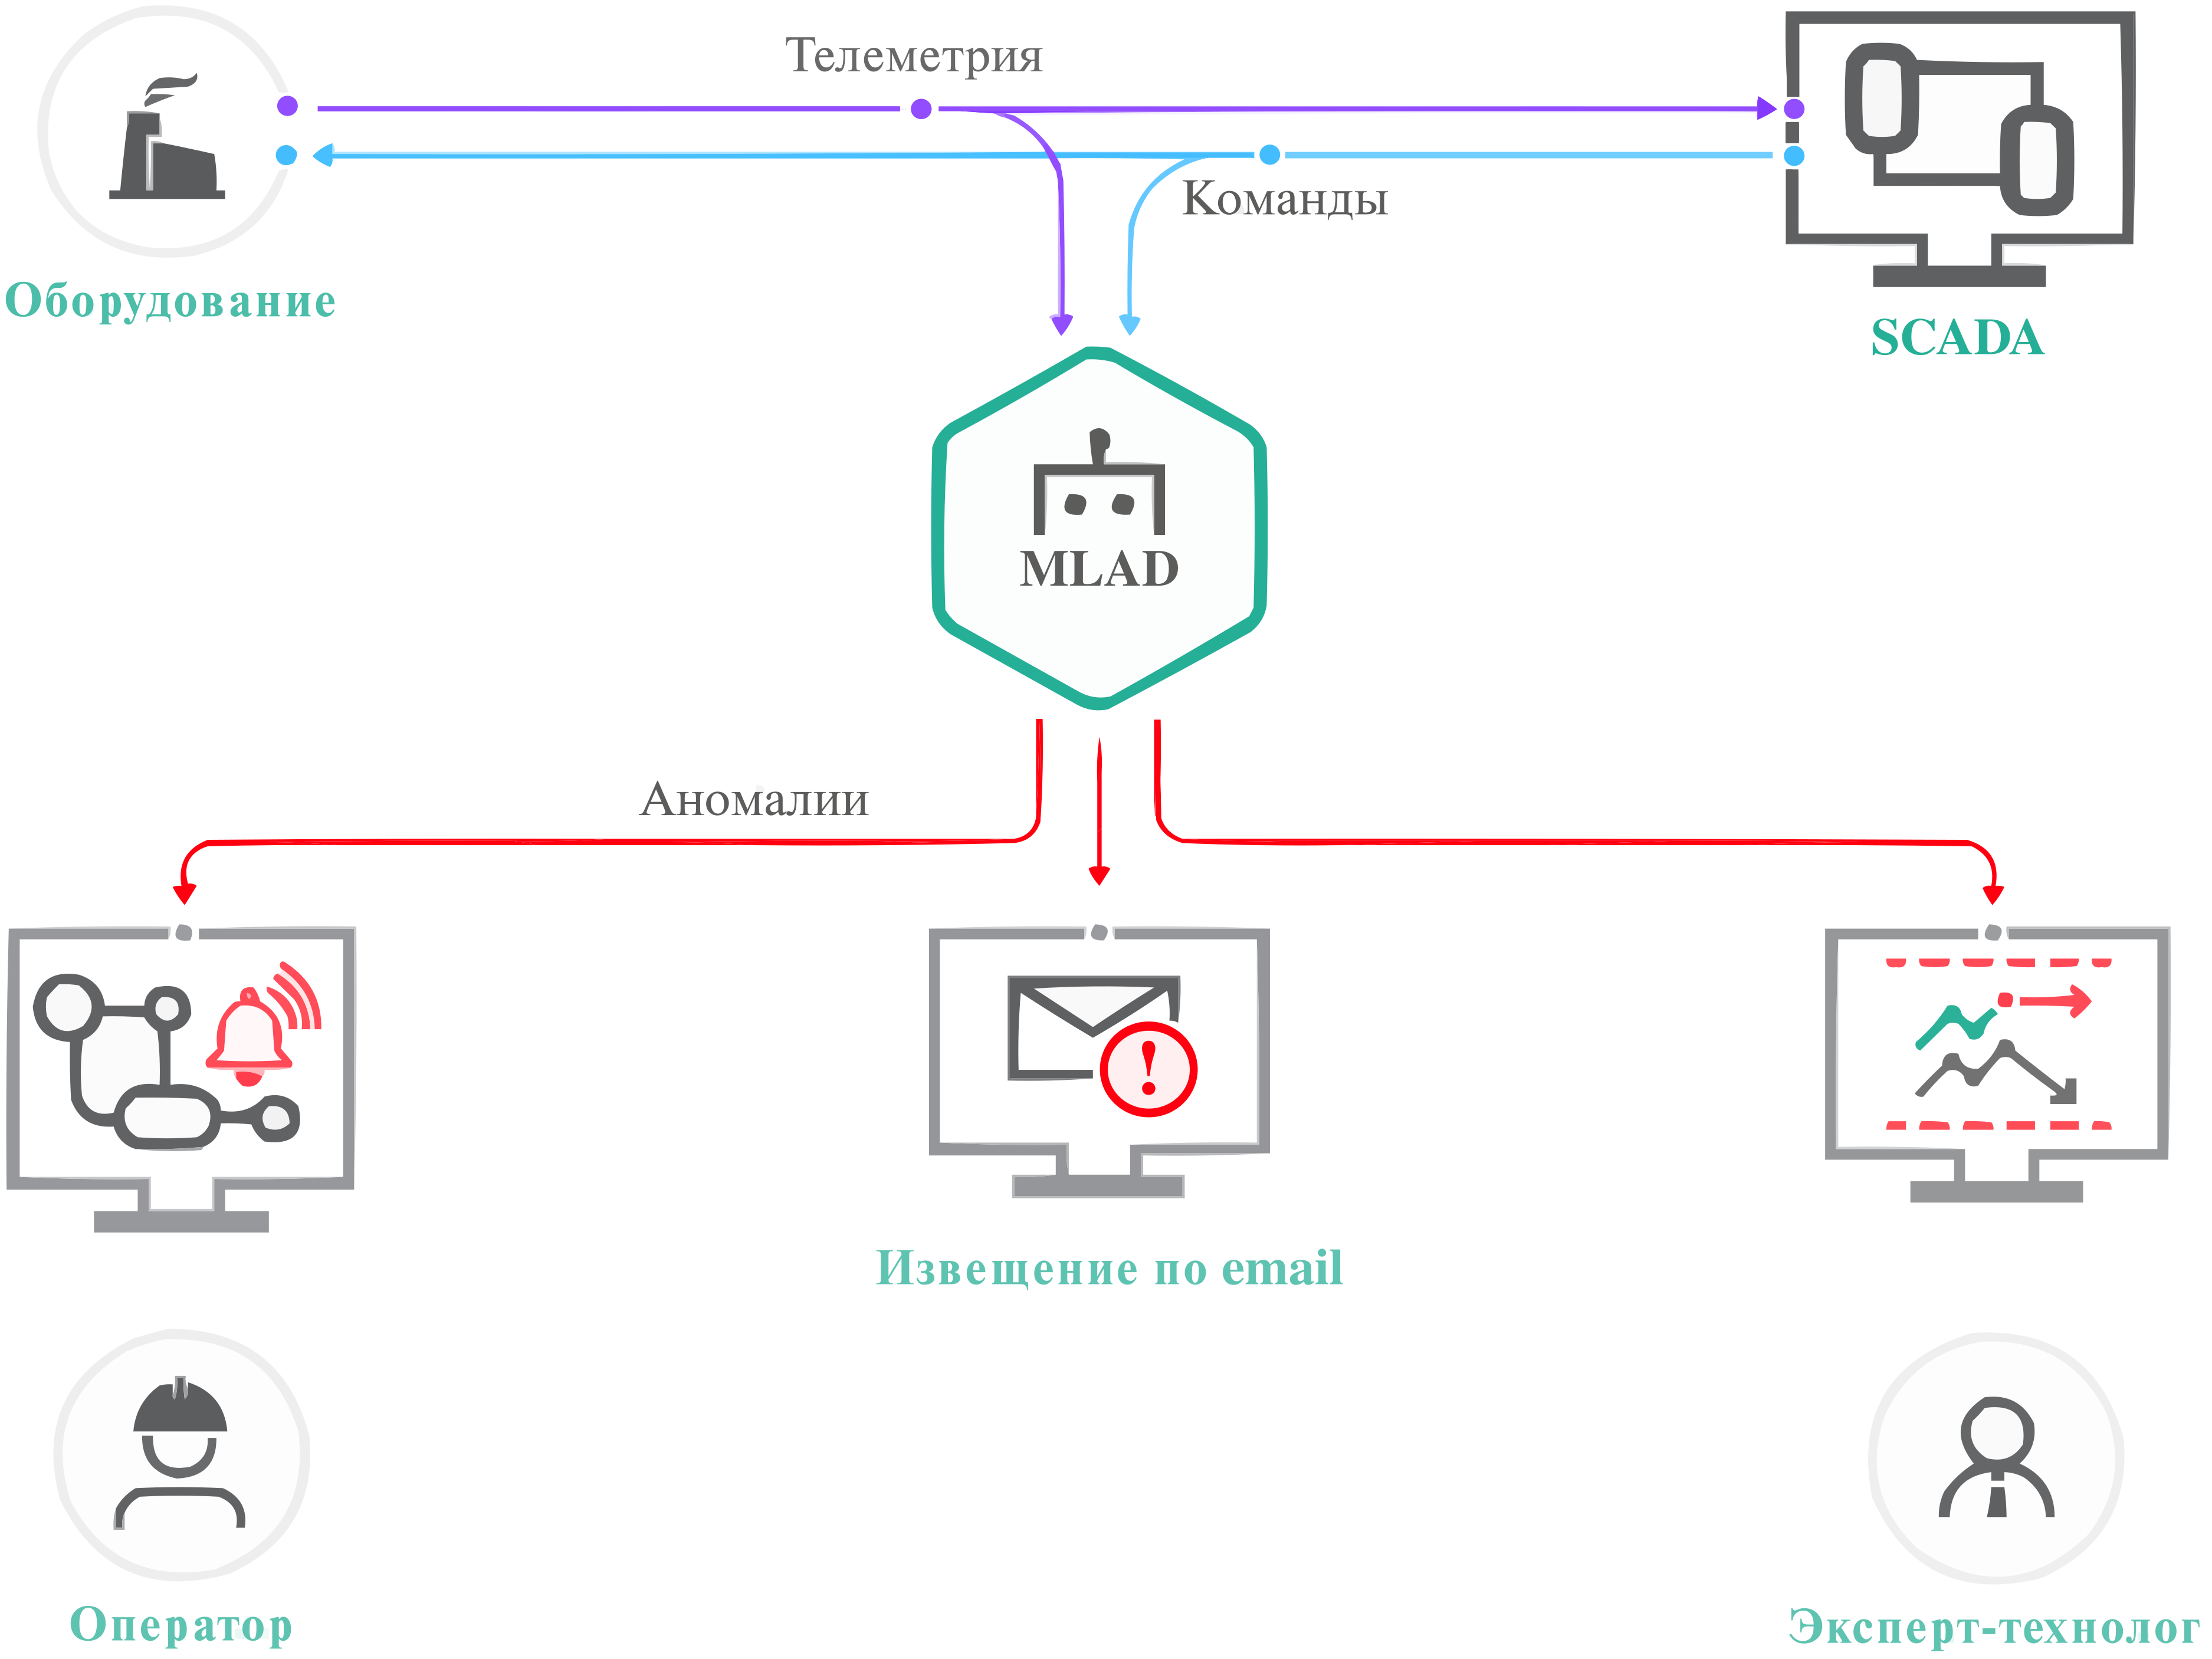
\includegraphics{images/chapter_3/Место_MLAD_на_производстве.png}
    \caption{Место системы Kaspersky MLAD на производстве}
    \label{fig:MLAD}
\end{figure}

Для работы системы Kaspersky MLAD не требуется изменять как-либо технологической процесс промышленного оборудования. Эта система никак не воздействует на него. К тому же она не вмешивается в передачу данных или в средства управления промышленным оборудованием. Данная система оповещает оператора о возможном сбое, и оставляет задачу принятия решения на операторе.

Если рассматривать Kaspersky MLAD с технической стороны, то это программное обеспечение, которое использует нейронные сети, способные анализировать существующий поток телеметрии. Поскольку параметры телеметрии связаны друг с другом и влияют друг на друга, то система Kaspersky MLAD должна это учитывать, и она с этим справляется. Она способна выявлять взаимосвязи между параметрами и использовать их для построения прогноза. Этот прогноз в дальнейшем обрабатывается различными нейросемантическими средствами, выявляя тем самым аномалии.

Система Kaspersky MLAD использует различные архитектуры нейронных сетей, такие как: CNN, DenseNet, TCN и RNN. Первые три сети используются для различного рода обработки данных, их анализа и выявление аномалий. А сети RNN используются для прогнозирования данных технологического процесса промышленного оборудования. Таким образом, Kaspersky MLAD состоит из различных модулей нейронных сетей, взаимодействующих друг с другом.

Но как именно система Kaspersky MLAD определяет аномалии. Для этого у системы имеется шесть видов детекторов аномалий или, если выражаться более правильно, аналитических процессоров:

\begin{itemize}
    \item предиктовый детектор;
    \item классификатор состояний;
    \item Детектор на основе диагностических правил;
    \item Детектор на основе прогноза времени до порога;
    \item потоковый процессов;
    \item процессор событий.
\end{itemize}

Предиктивный детектор аномалий есть система, которая сначала предсказывает текущие значения параметров объекта, после чего предсказание сравнивается с фактически наблюдаемым поведением. Если отклонение между реалным поведением процесса и предсказанным является значительным, тогда предиктовый детектор определяет это как аномалию. Детектор обучается по историческим данным телеметрии и выявляет аномалии «без подсказок» со стороны эксперта — в том числе и ранее неизвестные, никем не замеченные аномалии.

Классификатор состояний использует гауссовы модели, а если быть более точным, то алгоритм «эллиптический конверт». Этот детектор используются для автоматического выявления состояний объекта, которые значительно отличаются от состояний, соответствующих нормальным режимам работы.

Детектор на основе диагностических правил используется для выявления аномалий, симптомы которых заранее известны. Детектор отслеживает изменения в поведении объекта по заданным критериям. В диагностических правилах может быть реализована любая логика проверок. Наиболее популярные критерии: устойчивое превышение порога, рост или падение показателя за период, ступенчатый скачок, «замирание» значений на одном уровне.

Детектор на основе прогноза времени до порога также используется, чтобы предсказывать, когда тот или иной технологический параметр достигнет определенного порогового значения. Детектор срабатывает, когда времени до порога осталось меньше, чем указано в настройках.

Потоковый процессор приводит данные телеметрии, поступающие от объекта мониторинга в реальном времени, к равно-интервальной временной сетке, необходимой для работы предиктивных детекторов и диагностических правил. В процессе приведения данных к равно-интервальной временной сетке потоковый процессор выявляет и, по возможности, устраняет такие дефекты потока, как потерю данных, получение недостоверных значений, слишком раннее или слишком позднее прибытие наблюдений.

В отличие от предиктивного детектора, который анализирует непрерывные временные ряды, процессор событий работает с последовательностями дискретных событий. Специального вида нейронная сеть анализирует поток событий, выявляя типовые паттерны. Аномалией в данном случае является необычная последовательность событий, например, действия персонала и/или серия аномалий, выявленных другими детекторами.

Из всех видов детекторов подробнее стоит остановиться на предиктовом детекторе. Суть его работы проста: сначала выполняется прогноз данных, затем этот прогноз сравнивается с фактическим наблюдаемым поведением и с помощью машинного обучения определяются аномалии. Данный модуль можно разделить на две модели: модель прогнозирования и модель обработки прогнозов. Предиктовый детектор необходим для анализа данных технологического процесса, в основном представленных в виде временных рядов, содержащих разлиную информацию о состоянии объекта, различные физические величины, взятые с датчиков, и так далее. Предиктовый детектор работает по определённому алгоритму. Для начала формируется окно входных данных из поступивших на предиктовый детектор данных технологического процесса. На основе окна входных данных выполняется прогноз, формируя окно предсказания. Это окно показывает поведение объекта в определённом недалёком будущем. После вычисляется ошибка между прогнозом и реально наблюдаемыми данными для каждого предсказанного значения. Далее по совокупности этих ошибок производится вычисление среднеквадратичной ошибки. При вычислении этой ошибки значение индивидуальных ошибок прогноза умножаются на определённые веса. Таким образом осуществляется переход ко второй модели нейронной сети предиктового детектора. Этот модуль определяется по значению среднеквадратичной ошибки аномалию с помощью некоторого порога, который формируется при обучении модели нейронной сети. Пример данного процесса можно увидеть на рисунке \ref {fig:MLADex}.

\begin{figure}[H]
    \centering
    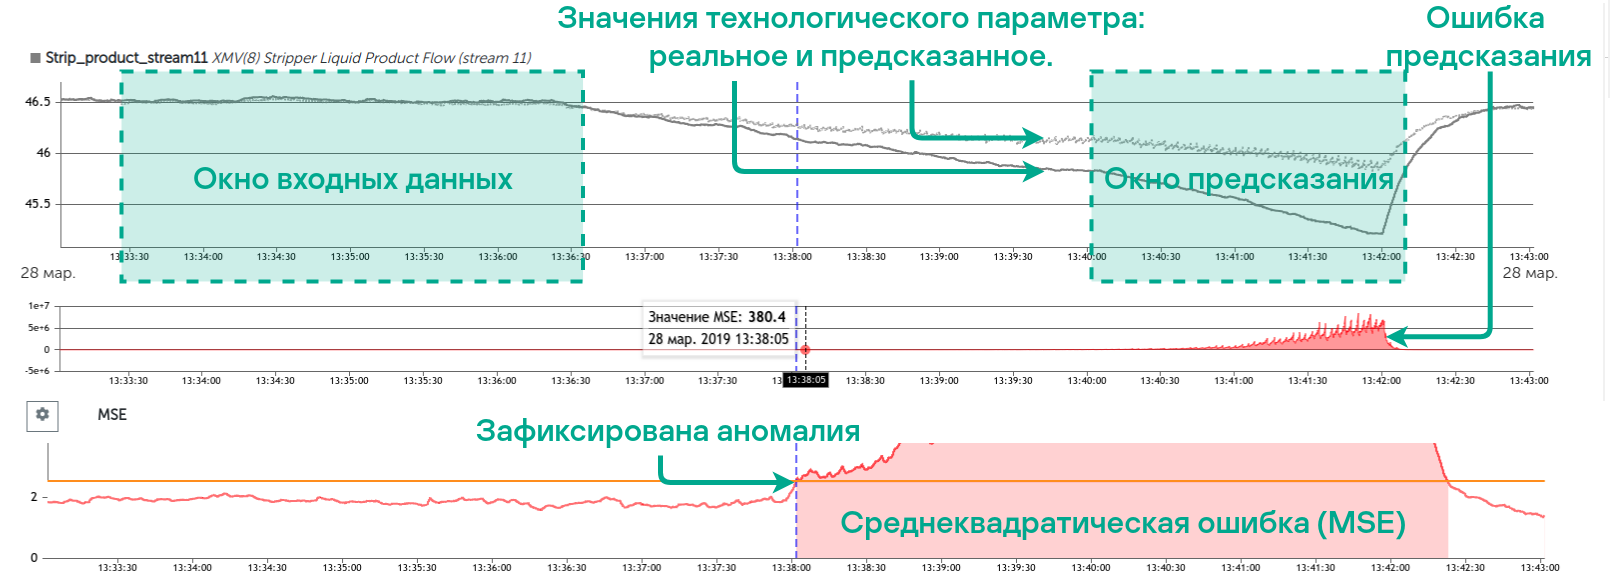
\includegraphics{images/chapter_3/MLAD_пример.png}
    \caption{Пример работы предиктового детектора системы Kaspersky MLAD}
    \label{fig:MLADex}
\end{figure}


\chapter{Заключение}

Задача повышения качества управления процессами в АСУТП является актуальной в настоящее время. Использование нейро-ПИД регулятора предложено как альтернатива другим самонастраивающимся схемам ПИД. Была разработана структура и алгоритм работы нейро-ПИД регулятора пастеризационной установки. Тестирование показало эффективность данной схемы.


\zlabel{lastpagetocount}

\chapter*{Библиографический список}
\addcontentsline{toc}{chapter}{Библиографический список}

\printbibliography[heading=subbibintoc, notkeyword={idzm}, title={Список использованных источников}]

\nocite{*}

\DeclareFieldFormat{labelnumberwidth}{#1\adddot\midsentence}
\newrefcontext[labelprefix={A-}, sorting=ynt]
\printbibliography[heading=subbibintoc, keyword={idzm}, title={Список публикаций соискателя}]


\end{document}
